%% HRFEST 2026 -- IEEE conference paper, camera-ready.
%% Every numerical value in the text comes from % Generated by scripts/make_numbers.py -- do not edit by hand.
% Every numeric value in main.tex comes from here.
\newcommand{\Ja}{1.50}
\newcommand{\backsteppingCICl}{[27, 43]}
\newcommand{\backsteppingCIInt}{[28, 44]}
\newcommand{\backsteppingCIMm}{[78, 91]}
\newcommand{\backsteppingCpu}{355}
\newcommand{\backsteppingCritOffsetCl}{1.0}
\newcommand{\backsteppingCritOffsetMm}{3.0}
\newcommand{\backsteppingFallTime}{8.1}
\newcommand{\backsteppingMcCl}{34.7}
\newcommand{\backsteppingMcInt}{35.3}
\newcommand{\backsteppingMcMm}{85.3}
\newcommand{\backsteppingMinOmegaCl}{n/a}
\newcommand{\backsteppingMinOmegaMm}{800}
\newcommand{\backsteppingNomBudget}{13}
\newcommand{\backsteppingNomSettle}{0.06}
\newcommand{\backsteppingRoaCl}{0}
\newcommand{\backsteppingRoaMm}{45}
\newcommand{\bpSurvivalSpread}{0}
\newcommand{\capacityAxis}{0.260}
\newcommand{\clSurvMaxOffset}{1.13}
\newcommand{\dtErr}{0.67}
\newcommand{\edge}{15}
\newcommand{\energyErr}{$8.9\times 10^{-13}$}
\newcommand{\etaFall}{0.83}
\newcommand{\etaLim}{0.831}
\newcommand{\etaPredErr}{3}
\newcommand{\etaPredErrNoise}{10}
\newcommand{\etaSlopeBks}{0.31}
\newcommand{\etaSlopeFbl}{0.34}
\newcommand{\etaSlopeLqr}{0.17}
\newcommand{\etaSlopePid}{0.20}
\newcommand{\etaSlopeSmc}{0.24}
\newcommand{\fblCICl}{[28, 44]}
\newcommand{\fblCIInt}{[28, 44]}
\newcommand{\fblCIMm}{[75, 88]}
\newcommand{\fblCpu}{354}
\newcommand{\fblCritOffsetCl}{1.0}
\newcommand{\fblCritOffsetMm}{3.0}
\newcommand{\fblFallTime}{8.2}
\newcommand{\fblFirstFallMm}{2.5}
\newcommand{\fblMcCl}{36.0}
\newcommand{\fblMcInt}{36.0}
\newcommand{\fblMcMm}{82.0}
\newcommand{\fblMinOmegaCl}{n/a}
\newcommand{\fblMinOmegaMm}{800}
\newcommand{\fblNomBudget}{17}
\newcommand{\fblNomSettle}{0.06}
\newcommand{\fblRoaCl}{0}
\newcommand{\fblRoaMm}{49}
\newcommand{\fs}{500}
\newcommand{\gravTorqueTen}{0.35}
\newcommand{\hmax}{0.150}
\newcommand{\hzDrift}{$1.1\times 10^{-11}$}
\newcommand{\jacErr}{$7.5\times 10^{-9}$}
\newcommand{\leanErr}{2}
\newcommand{\leanTwoMm}{0.64}
\newcommand{\lever}{14.6}
\newcommand{\lexBksMm}{98.0}
\newcommand{\lexBksP}{$p<10^{-4}$}
\newcommand{\lexClHi}{35.3}
\newcommand{\lexClLo}{31.3}
\newcommand{\lexFblMm}{96.0}
\newcommand{\lexFblP}{$p<10^{-4}$}
\newcommand{\lexLqrCl}{96.7}
\newcommand{\lexLqrP}{McNemar $p=0.12$}
\newcommand{\lexMpc}{96.7}
\newcommand{\lexPidMm}{98.7}
\newcommand{\lexSmcMm}{96.0}
\newcommand{\lqrCICl}{[96, 100]}
\newcommand{\lqrCIInt}{[81, 92]}
\newcommand{\lqrCIMm}{[97, 100]}
\newcommand{\lqrCpu}{189}
\newcommand{\lqrCritOffsetCl}{n/a}
\newcommand{\lqrCritOffsetMm}{n/a}
\newcommand{\lqrFallTime}{n/a}
\newcommand{\lqrKh}{0.002}
\newcommand{\lqrMcCl}{99.3}
\newcommand{\lqrMcInt}{87.3}
\newcommand{\lqrMcMm}{100.0}
\newcommand{\lqrMinOmegaCl}{400}
\newcommand{\lqrMinOmegaMm}{400}
\newcommand{\lqrNomBudget}{9}
\newcommand{\lqrNomSettle}{0.08}
\newcommand{\lqrRoaCl}{45}
\newcommand{\lqrRoaMm}{45}
\newcommand{\mass}{1.41}
\newcommand{\mcHorizon}{15}
\newcommand{\mcSeeds}{150}
\newcommand{\mmMinOmegaHi}{800}
\newcommand{\mmMinOmegaLo}{600}
\newcommand{\mpcCICl}{[92, 99]}
\newcommand{\mpcCpu}{221}
\newcommand{\mpcMcCl}{96.7}
\newcommand{\mpcNomBudget}{9}
\newcommand{\mpcNomSettle}{0.08}
\newcommand{\omegaTerm}{831}
\newcommand{\omegamax}{1000}
\newcommand{\pidCICl}{[26, 42]}
\newcommand{\pidCIInt}{[26, 42]}
\newcommand{\pidCIMm}{[92, 99]}
\newcommand{\pidCpu}{196}
\newcommand{\pidCritOffsetCl}{1.0}
\newcommand{\pidCritOffsetMm}{4.0}
\newcommand{\pidFallTime}{7.9}
\newcommand{\pidMcCl}{33.3}
\newcommand{\pidMcInt}{33.3}
\newcommand{\pidMcMm}{96.7}
\newcommand{\pidMinOmegaCl}{n/a}
\newcommand{\pidMinOmegaMm}{600}
\newcommand{\pidNomBudget}{14}
\newcommand{\pidNomSettle}{0.06}
\newcommand{\pidRoaCl}{0}
\newcommand{\pidRoaMm}{46}
\newcommand{\roaBlindCl}{0}
\newcommand{\roaPerpCl}{16}
\newcommand{\roaPerpHigh}{49}
\newcommand{\roaPerpMm}{50}
\newcommand{\roaPerpZero}{50}
\newcommand{\roaVertCl}{14}
\newcommand{\roaVertHigh}{34}
\newcommand{\roaVertMm}{42}
\newcommand{\roaVertZero}{50}
\newcommand{\satTime}{0.43}
\newcommand{\smcCICl}{[28, 44]}
\newcommand{\smcCIInt}{[28, 44]}
\newcommand{\smcCIMm}{[88, 97]}
\newcommand{\smcCpu}{365}
\newcommand{\smcCritOffsetCl}{1.0}
\newcommand{\smcCritOffsetMm}{4.0}
\newcommand{\smcFallTime}{8.2}
\newcommand{\smcMcCl}{36.0}
\newcommand{\smcMcInt}{36.0}
\newcommand{\smcMcMm}{94.0}
\newcommand{\smcMinOmegaCl}{n/a}
\newcommand{\smcMinOmegaMm}{600}
\newcommand{\smcNomBudget}{12}
\newcommand{\smcNomSettle}{0.06}
\newcommand{\smcRoaCl}{0}
\newcommand{\smcRoaMm}{46}
\newcommand{\swingBalanced}{0/5}
\newcommand{\swingGamma}{0.07}
\newcommand{\taumax}{0.50}
\newcommand{\tsatPred}{15.6}
\newcommand{\tsatSlope}{16.5}
, which is
%% generated by scripts/make_numbers.py from the CSV files in results/.
%% No number is typed by hand.
\documentclass[conference]{IEEEtran}
\IEEEoverridecommandlockouts

\usepackage{cite}
\usepackage{amsmath,amssymb,amsfonts}
\usepackage{amsthm}
\usepackage{algorithmic}
\usepackage{graphicx}
\usepackage{textcomp}
\usepackage{xcolor}
\usepackage{booktabs}
\usepackage{enumitem}
\usepackage{float}
\usepackage{siunitx}
\newcommand{\PaperTitle}{Gravity-Torque Momentum Management for a Three-Wheel Reaction-Wheel Inverted Pendulum}
\newcommand{\PaperAuthors}{Jose Luis Segundo Manayay, Javier Yanpier Garay Yovera, Francisco Jes\'us Rodr\'iguez Huiman}
\newcommand{\PaperAuthorsPDF}{Jose Luis Segundo Manayay, Javier Yanpier Garay Yovera, Francisco Jes\string\372s Rodr\string\355guez Huiman}
\usepackage{url}
% PDF profiles from one source.
%   interactive: blue mailto/DOI/URL links and a clickable ORCID logo.
%   ieee (default): no link annotations and no bookmarks, for IEEE PDF eXpress;
%   metadata written with \pdfinfo; ORCID logo kept as plain vector art.
% Select with \def\PDFPROFILE{interactive} before %% HRFEST 2026 -- IEEE conference paper, camera-ready.
%% Every numerical value in the text comes from % Generated by scripts/make_numbers.py -- do not edit by hand.
% Every numeric value in main.tex comes from here.
\newcommand{\Ja}{1.50}
\newcommand{\backsteppingCICl}{[27, 43]}
\newcommand{\backsteppingCIInt}{[28, 44]}
\newcommand{\backsteppingCIMm}{[78, 91]}
\newcommand{\backsteppingCpu}{355}
\newcommand{\backsteppingCritOffsetCl}{1.0}
\newcommand{\backsteppingCritOffsetMm}{3.0}
\newcommand{\backsteppingFallTime}{8.1}
\newcommand{\backsteppingMcCl}{34.7}
\newcommand{\backsteppingMcInt}{35.3}
\newcommand{\backsteppingMcMm}{85.3}
\newcommand{\backsteppingMinOmegaCl}{n/a}
\newcommand{\backsteppingMinOmegaMm}{800}
\newcommand{\backsteppingNomBudget}{13}
\newcommand{\backsteppingNomSettle}{0.06}
\newcommand{\backsteppingRoaCl}{0}
\newcommand{\backsteppingRoaMm}{45}
\newcommand{\bpSurvivalSpread}{0}
\newcommand{\capacityAxis}{0.260}
\newcommand{\clSurvMaxOffset}{1.13}
\newcommand{\dtErr}{0.67}
\newcommand{\edge}{15}
\newcommand{\energyErr}{$8.9\times 10^{-13}$}
\newcommand{\etaFall}{0.83}
\newcommand{\etaLim}{0.831}
\newcommand{\etaPredErr}{3}
\newcommand{\etaPredErrNoise}{10}
\newcommand{\etaSlopeBks}{0.31}
\newcommand{\etaSlopeFbl}{0.34}
\newcommand{\etaSlopeLqr}{0.17}
\newcommand{\etaSlopePid}{0.20}
\newcommand{\etaSlopeSmc}{0.24}
\newcommand{\fblCICl}{[28, 44]}
\newcommand{\fblCIInt}{[28, 44]}
\newcommand{\fblCIMm}{[75, 88]}
\newcommand{\fblCpu}{354}
\newcommand{\fblCritOffsetCl}{1.0}
\newcommand{\fblCritOffsetMm}{3.0}
\newcommand{\fblFallTime}{8.2}
\newcommand{\fblFirstFallMm}{2.5}
\newcommand{\fblMcCl}{36.0}
\newcommand{\fblMcInt}{36.0}
\newcommand{\fblMcMm}{82.0}
\newcommand{\fblMinOmegaCl}{n/a}
\newcommand{\fblMinOmegaMm}{800}
\newcommand{\fblNomBudget}{17}
\newcommand{\fblNomSettle}{0.06}
\newcommand{\fblRoaCl}{0}
\newcommand{\fblRoaMm}{49}
\newcommand{\fs}{500}
\newcommand{\gravTorqueTen}{0.35}
\newcommand{\hmax}{0.150}
\newcommand{\hzDrift}{$1.1\times 10^{-11}$}
\newcommand{\jacErr}{$7.5\times 10^{-9}$}
\newcommand{\leanErr}{2}
\newcommand{\leanTwoMm}{0.64}
\newcommand{\lever}{14.6}
\newcommand{\lexBksMm}{98.0}
\newcommand{\lexBksP}{$p<10^{-4}$}
\newcommand{\lexClHi}{35.3}
\newcommand{\lexClLo}{31.3}
\newcommand{\lexFblMm}{96.0}
\newcommand{\lexFblP}{$p<10^{-4}$}
\newcommand{\lexLqrCl}{96.7}
\newcommand{\lexLqrP}{McNemar $p=0.12$}
\newcommand{\lexMpc}{96.7}
\newcommand{\lexPidMm}{98.7}
\newcommand{\lexSmcMm}{96.0}
\newcommand{\lqrCICl}{[96, 100]}
\newcommand{\lqrCIInt}{[81, 92]}
\newcommand{\lqrCIMm}{[97, 100]}
\newcommand{\lqrCpu}{189}
\newcommand{\lqrCritOffsetCl}{n/a}
\newcommand{\lqrCritOffsetMm}{n/a}
\newcommand{\lqrFallTime}{n/a}
\newcommand{\lqrKh}{0.002}
\newcommand{\lqrMcCl}{99.3}
\newcommand{\lqrMcInt}{87.3}
\newcommand{\lqrMcMm}{100.0}
\newcommand{\lqrMinOmegaCl}{400}
\newcommand{\lqrMinOmegaMm}{400}
\newcommand{\lqrNomBudget}{9}
\newcommand{\lqrNomSettle}{0.08}
\newcommand{\lqrRoaCl}{45}
\newcommand{\lqrRoaMm}{45}
\newcommand{\mass}{1.41}
\newcommand{\mcHorizon}{15}
\newcommand{\mcSeeds}{150}
\newcommand{\mmMinOmegaHi}{800}
\newcommand{\mmMinOmegaLo}{600}
\newcommand{\mpcCICl}{[92, 99]}
\newcommand{\mpcCpu}{221}
\newcommand{\mpcMcCl}{96.7}
\newcommand{\mpcNomBudget}{9}
\newcommand{\mpcNomSettle}{0.08}
\newcommand{\omegaTerm}{831}
\newcommand{\omegamax}{1000}
\newcommand{\pidCICl}{[26, 42]}
\newcommand{\pidCIInt}{[26, 42]}
\newcommand{\pidCIMm}{[92, 99]}
\newcommand{\pidCpu}{196}
\newcommand{\pidCritOffsetCl}{1.0}
\newcommand{\pidCritOffsetMm}{4.0}
\newcommand{\pidFallTime}{7.9}
\newcommand{\pidMcCl}{33.3}
\newcommand{\pidMcInt}{33.3}
\newcommand{\pidMcMm}{96.7}
\newcommand{\pidMinOmegaCl}{n/a}
\newcommand{\pidMinOmegaMm}{600}
\newcommand{\pidNomBudget}{14}
\newcommand{\pidNomSettle}{0.06}
\newcommand{\pidRoaCl}{0}
\newcommand{\pidRoaMm}{46}
\newcommand{\roaBlindCl}{0}
\newcommand{\roaPerpCl}{16}
\newcommand{\roaPerpHigh}{49}
\newcommand{\roaPerpMm}{50}
\newcommand{\roaPerpZero}{50}
\newcommand{\roaVertCl}{14}
\newcommand{\roaVertHigh}{34}
\newcommand{\roaVertMm}{42}
\newcommand{\roaVertZero}{50}
\newcommand{\satTime}{0.43}
\newcommand{\smcCICl}{[28, 44]}
\newcommand{\smcCIInt}{[28, 44]}
\newcommand{\smcCIMm}{[88, 97]}
\newcommand{\smcCpu}{365}
\newcommand{\smcCritOffsetCl}{1.0}
\newcommand{\smcCritOffsetMm}{4.0}
\newcommand{\smcFallTime}{8.2}
\newcommand{\smcMcCl}{36.0}
\newcommand{\smcMcInt}{36.0}
\newcommand{\smcMcMm}{94.0}
\newcommand{\smcMinOmegaCl}{n/a}
\newcommand{\smcMinOmegaMm}{600}
\newcommand{\smcNomBudget}{12}
\newcommand{\smcNomSettle}{0.06}
\newcommand{\smcRoaCl}{0}
\newcommand{\smcRoaMm}{46}
\newcommand{\swingBalanced}{0/5}
\newcommand{\swingGamma}{0.07}
\newcommand{\taumax}{0.50}
\newcommand{\tsatPred}{15.6}
\newcommand{\tsatSlope}{16.5}
, which is
%% generated by scripts/make_numbers.py from the CSV files in results/.
%% No number is typed by hand.
\documentclass[conference]{IEEEtran}
\IEEEoverridecommandlockouts

\usepackage{cite}
\usepackage{amsmath,amssymb,amsfonts}
\usepackage{amsthm}
\usepackage{algorithmic}
\usepackage{graphicx}
\usepackage{textcomp}
\usepackage{xcolor}
\usepackage{booktabs}
\usepackage{enumitem}
\usepackage{float}
\usepackage{siunitx}
\newcommand{\PaperTitle}{Gravity-Torque Momentum Management for a Three-Wheel Reaction-Wheel Inverted Pendulum}
\newcommand{\PaperAuthors}{Jose Luis Segundo Manayay, Javier Yanpier Garay Yovera, Francisco Jes\'us Rodr\'iguez Huiman}
\newcommand{\PaperAuthorsPDF}{Jose Luis Segundo Manayay, Javier Yanpier Garay Yovera, Francisco Jes\string\372s Rodr\string\355guez Huiman}
\usepackage{url}
% PDF profiles from one source.
%   interactive: blue mailto/DOI/URL links and a clickable ORCID logo.
%   ieee (default): no link annotations and no bookmarks, for IEEE PDF eXpress;
%   metadata written with \pdfinfo; ORCID logo kept as plain vector art.
% Select with \def\PDFPROFILE{interactive} before \input{main.tex}.
% Requires \PaperTitle, \PaperAuthors (UTF-8, hyperref) and \PaperAuthorsPDF
% (PDFDocEncoding octal escapes, \pdfinfo) to be defined first.
\ifdefined\PDFPROFILE\else\def\PDFPROFILE{ieee}\fi
\def\profileinteractive{interactive}
\usepackage{tikz}
\usetikzlibrary{svg.path}
\definecolor{orcidlogocol}{HTML}{A6CE39}
% ORCID iD logo, same artwork as the orcidlink package (vector, no Type 3).
\newlength{\orcidxheight}
\newcommand{\orcidlogo}{\setlength{\orcidxheight}{\fontcharht\font`X}%
  \mbox{\begin{tikzpicture}[yscale=-0.00390625*\orcidxheight,
      xscale=0.00390625*\orcidxheight,transform shape]
    \fill[orcidlogocol] svg{M256,128c0,70.7-57.3,128-128,128C57.3,256,0,198.7,0,128C0,57.3,57.3,0,128,0C198.7,0,256,57.3,256,128z};
    \fill[white] svg{M86.3,186.2H70.9V79.1h15.4v48.4V186.2z}
      svg{M108.9,79.1h41.6c39.6,0,57,28.3,57,53.6c0,27.5-21.5,53.6-56.8,53.6h-41.8V79.1z M124.3,172.4h24.5c34.9,0,42.9-26.5,42.9-39.7c0-21.5-13.7-39.7-43.7-39.7h-23.7V172.4z}
      svg{M88.7,56.8c0,5.5-4.5,10.1-10.1,10.1c-5.6,0-10.1-4.6-10.1-10.1c0-5.6,4.5-10.1,10.1-10.1C84.2,46.7,88.7,51.3,88.7,56.8z};
  \end{tikzpicture}}}
\ifx\PDFPROFILE\profileinteractive
  \usepackage[colorlinks=true,linkcolor=black,citecolor=black,urlcolor=blue,
              bookmarks=false]{hyperref}
  \hypersetup{pdftitle={\PaperTitle},pdfauthor={\PaperAuthors}}
  \newcommand{\orcid}[1]{\href{https://orcid.org/#1}{\orcidlogo}}
  \newcommand{\authoremail}[1]{\href{mailto:#1}{#1}}
  \newcommand{\doititle}[2]{\href{https://doi.org/#1}{#2}}
  \newcommand{\urltitle}[2]{\href{#1}{#2}}
\else
  \pdfinfo{/Title (\PaperTitle) /Author (\PaperAuthorsPDF)}
  \newcommand{\orcid}[1]{\orcidlogo}
  \newcommand{\authoremail}[1]{#1}
  \newcommand{\doititle}[2]{#2}
  \newcommand{\urltitle}[2]{#2}
\fi

\usetikzlibrary{patterns,positioning}
% Coauthor ORCID iDs (found in the BLADE_mars_coaxial CITATION.cff and on
% orcid.org) are shown only after each coauthor confirms them personally.
\newif\ifcoauthororcid \coauthororcidtrue
\newcommand{\coorcid}[1]{\ifcoauthororcid\,\orcid{#1}\fi}
% Affiliation confirmed by the corresponding author (2026-10-23) for all authors.
\newcommand{\paperaffiliation}{Universidad Nacional de Ingenier\'ia (UNI), Faculty of
  Mechanical Engineering, Lima, Peru}


\def\BibTeX{{\rm B\kern-.05em{\sc i\kern-.025em b}\kern-.08em T\kern-.1667em\lower.7ex\hbox{E}\kern-.125emX}}

\newtheorem{lemma}{Lemma}
\newtheorem{theorem}{Theorem}
\newtheorem{proposition}{Proposition}
\theoremstyle{definition}
\newtheorem{definition}{Definition}
\theoremstyle{plain}
\newtheorem{corollary}{Corollary}
\newtheorem{remark}{Remark}

\newcommand{\R}{\mathbb{R}}
\newcommand{\SO}{\mathrm{SO}(3)}
\newcommand{\skewm}[1]{\left[#1\right]_\times}
\newcommand{\bw}{\boldsymbol{\omega}}
\newcommand{\bOm}{\boldsymbol{\Omega}}
\newcommand{\btau}{\boldsymbol{\tau}}
\newcommand{\bh}{\boldsymbol{h}}
\newcommand{\bJ}{\boldsymbol{J}}
\newcommand{\bn}{\boldsymbol{n}}
\newcommand{\bre}{\boldsymbol{r}}
\newcommand{\btheta}{\boldsymbol{\theta}}

% Generated by scripts/make_numbers.py -- do not edit by hand.
% Every numeric value in main.tex comes from here.
\newcommand{\Ja}{1.50}
\newcommand{\backsteppingCICl}{[27, 43]}
\newcommand{\backsteppingCIInt}{[28, 44]}
\newcommand{\backsteppingCIMm}{[78, 91]}
\newcommand{\backsteppingCpu}{355}
\newcommand{\backsteppingCritOffsetCl}{1.0}
\newcommand{\backsteppingCritOffsetMm}{3.0}
\newcommand{\backsteppingFallTime}{8.1}
\newcommand{\backsteppingMcCl}{34.7}
\newcommand{\backsteppingMcInt}{35.3}
\newcommand{\backsteppingMcMm}{85.3}
\newcommand{\backsteppingMinOmegaCl}{n/a}
\newcommand{\backsteppingMinOmegaMm}{800}
\newcommand{\backsteppingNomBudget}{13}
\newcommand{\backsteppingNomSettle}{0.06}
\newcommand{\backsteppingRoaCl}{0}
\newcommand{\backsteppingRoaMm}{45}
\newcommand{\bpSurvivalSpread}{0}
\newcommand{\capacityAxis}{0.260}
\newcommand{\clSurvMaxOffset}{1.13}
\newcommand{\dtErr}{0.67}
\newcommand{\edge}{15}
\newcommand{\energyErr}{$8.9\times 10^{-13}$}
\newcommand{\etaFall}{0.83}
\newcommand{\etaLim}{0.831}
\newcommand{\etaPredErr}{3}
\newcommand{\etaPredErrNoise}{10}
\newcommand{\etaSlopeBks}{0.31}
\newcommand{\etaSlopeFbl}{0.34}
\newcommand{\etaSlopeLqr}{0.17}
\newcommand{\etaSlopePid}{0.20}
\newcommand{\etaSlopeSmc}{0.24}
\newcommand{\fblCICl}{[28, 44]}
\newcommand{\fblCIInt}{[28, 44]}
\newcommand{\fblCIMm}{[75, 88]}
\newcommand{\fblCpu}{354}
\newcommand{\fblCritOffsetCl}{1.0}
\newcommand{\fblCritOffsetMm}{3.0}
\newcommand{\fblFallTime}{8.2}
\newcommand{\fblFirstFallMm}{2.5}
\newcommand{\fblMcCl}{36.0}
\newcommand{\fblMcInt}{36.0}
\newcommand{\fblMcMm}{82.0}
\newcommand{\fblMinOmegaCl}{n/a}
\newcommand{\fblMinOmegaMm}{800}
\newcommand{\fblNomBudget}{17}
\newcommand{\fblNomSettle}{0.06}
\newcommand{\fblRoaCl}{0}
\newcommand{\fblRoaMm}{49}
\newcommand{\fs}{500}
\newcommand{\gravTorqueTen}{0.35}
\newcommand{\hmax}{0.150}
\newcommand{\hzDrift}{$1.1\times 10^{-11}$}
\newcommand{\jacErr}{$7.5\times 10^{-9}$}
\newcommand{\leanErr}{2}
\newcommand{\leanTwoMm}{0.64}
\newcommand{\lever}{14.6}
\newcommand{\lexBksMm}{98.0}
\newcommand{\lexBksP}{$p<10^{-4}$}
\newcommand{\lexClHi}{35.3}
\newcommand{\lexClLo}{31.3}
\newcommand{\lexFblMm}{96.0}
\newcommand{\lexFblP}{$p<10^{-4}$}
\newcommand{\lexLqrCl}{96.7}
\newcommand{\lexLqrP}{McNemar $p=0.12$}
\newcommand{\lexMpc}{96.7}
\newcommand{\lexPidMm}{98.7}
\newcommand{\lexSmcMm}{96.0}
\newcommand{\lqrCICl}{[96, 100]}
\newcommand{\lqrCIInt}{[81, 92]}
\newcommand{\lqrCIMm}{[97, 100]}
\newcommand{\lqrCpu}{189}
\newcommand{\lqrCritOffsetCl}{n/a}
\newcommand{\lqrCritOffsetMm}{n/a}
\newcommand{\lqrFallTime}{n/a}
\newcommand{\lqrKh}{0.002}
\newcommand{\lqrMcCl}{99.3}
\newcommand{\lqrMcInt}{87.3}
\newcommand{\lqrMcMm}{100.0}
\newcommand{\lqrMinOmegaCl}{400}
\newcommand{\lqrMinOmegaMm}{400}
\newcommand{\lqrNomBudget}{9}
\newcommand{\lqrNomSettle}{0.08}
\newcommand{\lqrRoaCl}{45}
\newcommand{\lqrRoaMm}{45}
\newcommand{\mass}{1.41}
\newcommand{\mcHorizon}{15}
\newcommand{\mcSeeds}{150}
\newcommand{\mmMinOmegaHi}{800}
\newcommand{\mmMinOmegaLo}{600}
\newcommand{\mpcCICl}{[92, 99]}
\newcommand{\mpcCpu}{221}
\newcommand{\mpcMcCl}{96.7}
\newcommand{\mpcNomBudget}{9}
\newcommand{\mpcNomSettle}{0.08}
\newcommand{\omegaTerm}{831}
\newcommand{\omegamax}{1000}
\newcommand{\pidCICl}{[26, 42]}
\newcommand{\pidCIInt}{[26, 42]}
\newcommand{\pidCIMm}{[92, 99]}
\newcommand{\pidCpu}{196}
\newcommand{\pidCritOffsetCl}{1.0}
\newcommand{\pidCritOffsetMm}{4.0}
\newcommand{\pidFallTime}{7.9}
\newcommand{\pidMcCl}{33.3}
\newcommand{\pidMcInt}{33.3}
\newcommand{\pidMcMm}{96.7}
\newcommand{\pidMinOmegaCl}{n/a}
\newcommand{\pidMinOmegaMm}{600}
\newcommand{\pidNomBudget}{14}
\newcommand{\pidNomSettle}{0.06}
\newcommand{\pidRoaCl}{0}
\newcommand{\pidRoaMm}{46}
\newcommand{\roaBlindCl}{0}
\newcommand{\roaPerpCl}{16}
\newcommand{\roaPerpHigh}{49}
\newcommand{\roaPerpMm}{50}
\newcommand{\roaPerpZero}{50}
\newcommand{\roaVertCl}{14}
\newcommand{\roaVertHigh}{34}
\newcommand{\roaVertMm}{42}
\newcommand{\roaVertZero}{50}
\newcommand{\satTime}{0.43}
\newcommand{\smcCICl}{[28, 44]}
\newcommand{\smcCIInt}{[28, 44]}
\newcommand{\smcCIMm}{[88, 97]}
\newcommand{\smcCpu}{365}
\newcommand{\smcCritOffsetCl}{1.0}
\newcommand{\smcCritOffsetMm}{4.0}
\newcommand{\smcFallTime}{8.2}
\newcommand{\smcMcCl}{36.0}
\newcommand{\smcMcInt}{36.0}
\newcommand{\smcMcMm}{94.0}
\newcommand{\smcMinOmegaCl}{n/a}
\newcommand{\smcMinOmegaMm}{600}
\newcommand{\smcNomBudget}{12}
\newcommand{\smcNomSettle}{0.06}
\newcommand{\smcRoaCl}{0}
\newcommand{\smcRoaMm}{46}
\newcommand{\swingBalanced}{0/5}
\newcommand{\swingGamma}{0.07}
\newcommand{\taumax}{0.50}
\newcommand{\tsatPred}{15.6}
\newcommand{\tsatSlope}{16.5}


\renewcommand{\topfraction}{0.92}
\renewcommand{\bottomfraction}{0.85}
\renewcommand{\textfraction}{0.07}
\renewcommand{\floatpagefraction}{0.80}
\setlength{\textfloatsep}{7pt plus 2pt minus 2pt}
\setlength{\floatsep}{7pt plus 2pt minus 2pt}
\setlength{\intextsep}{7pt plus 2pt minus 2pt}
\setlength{\abovecaptionskip}{3pt}
\setlength{\belowcaptionskip}{0pt}

\begin{document}

\title{Gravity-Torque Momentum Management for a\\
Three-Wheel Reaction-Wheel Inverted Pendulum}

\author{\IEEEauthorblockN{Jose Luis Segundo Manayay\textsuperscript{*}\,\orcid{0009-0002-9203-8710},
Javier Yanpier Garay Yovera\coorcid{0009-0001-1645-8724},
Francisco Jes\'us Rodr\'iguez Huiman\coorcid{0009-0006-6972-2484}}
\IEEEauthorblockA{\paperaffiliation\\
\authoremail{jose.segundo.m@uni.pe}; \authoremail{javier.garay.y@uni.pe}; \authoremail{francisco.rodriguez.h@uni.pe}\\
{\footnotesize $^{*}$Corresponding author}}}

\maketitle
\raggedbottom

\begin{abstract}
A reaction wheel that holds a body against a persistent torque integrates that
torque, so its speed, not its torque, is what runs out. On a pendulum balancing
about a ground pivot the only external torque that can unload the wheels is
gravity, which also destabilizes the plant. We show that any equilibrium of the
disturbed plant holds the attitude at which gravity balances the disturbance,
with no momentum accumulating in the wheels, so designs that regulate the
attitude error to zero have no equilibrium to reach. A \SI{2}{\milli\metre}
center-of-mass offset needs under \SI{1}{\degree} of lean, yet it fells
feedback linearization, sliding mode control, backstepping and PID, and an
integrator on the attitude error does not help. On a nonlinear three-wheel
model with a torque--speed envelope, a digital loop and sensor noise, over
\mcSeeds{} simulated plants with random center-of-mass offsets and a
\mcHorizon\,\si{\second} horizon, these
designs balance \pidMcCl--\fblMcCl\,\si{\percent} of the plants; a
gravity-torque unloading augmentation raises them to
\fblMcMm--\pidMcMm\,\si{\percent}; the best is level with a constrained
MPC (\mpcMcCl\,\si{\percent}), and none outperforms it or an LQR weighted on
stored momentum (\lqrMcCl\,\si{\percent}).
\end{abstract}

\begin{IEEEkeywords}
underactuated systems, reaction wheels, inverted pendulum, momentum management,
actuator constraints, model predictive control, sliding mode control,
backstepping
\end{IEEEkeywords}

\section{Introduction}
\label{sec:intro}

The reaction-wheel pendulum is a standard benchmark for nonlinear
control~\cite{spong2001}, and the Cubli~\cite{gajamohan2013,muehlebach2017}
extends it to balancing a cube on one vertex with three orthogonal wheels;
comparisons of LQR, feedback linearization, sliding mode control and
backstepping on this plant are common~\cite{wasiwitono2025}. They usually model
the actuator as a torque saturation. A wheel that holds a body against a
persistent torque, however, \emph{integrates} it, and its speed grows until no
reaction torque is left in that direction; wheel-speed excess is the reported
failure mode on a Cubli-type rover~\cite{huang2022}.

Spacecraft handle this with momentum management~\cite{sidi1997}, unloading the
wheels through an external torque~\cite{powell1972} or constraining wheel
momentum directly~\cite{alipour2025}. For balancing machines, the invariance of
the Cubli's vertical momentum is known~\cite{muehlebach2017}, a ballbot holds a
center-of-mass offset by leaning~\cite{vaidya2015ballbot}, a reaction-wheel
bicycle balances under lateral load~\cite{huang2025bicycle}, and reference
governors enforce constraints through set-points~\cite{garone2017governors}.
What is specific to a body balancing about a ground pivot is that the only
unloading torque is the \emph{same first-order gravity torque} that
destabilizes it: in orbit unloading costs pointing accuracy, here it costs
stability margin.

We ask which designs keep such a pendulum balanced under a persistent
disturbance when wheel speed, not torque, is the binding limit, and contribute:
(i)~an equilibrium condition (Proposition~\ref{prop:lean}): every equilibrium of
the disturbed plant holds a gravity-balanced lean, to first order
$\|P\btau_d\|/(Mgl)$, so designs regulating $\btheta_e\!\to\!0$ have no
equilibrium to reach; (ii)~a directional capacity bound
(Proposition~\ref{prop:capacity}; cf.~\cite{markley2009envelopes}) that corrects
the scalar budget by $\|\bn\|_1$; (iii)~a measurement of which limit binds:
classical designs fail at $\eta_\Omega\approx\etaFall$, where the accelerating
envelope no longer covers bearing friction; and (iv)~a comparison of five
designs, each classical, with integral action and with momentum management,
against a constrained MPC, all tuned by one protocol
(Secs.~\ref{sec:control}--\ref{sec:results}).

\section{Problem Formulation}
\label{sec:model}

\subsection{Geometry and states}

The testbed is a cube of edge $L$ carrying three identical reaction wheels
whose spin axes coincide with the body axes $\bre_1,\bre_2,\bre_3$
(Fig.~\ref{fig:system}). It pivots about one vertex, treated as an ideal
spherical joint. Let $R\in\SO$ rotate body coordinates into the inertial
frame, $\bw\in\R^3$ be the body angular velocity, and $\bOm\in\R^3$ collect
the wheel speeds \emph{relative to the body}.

Let $\bJ$ be the inertia of the whole assembly about the pivot, wheels
included as if rigidly attached, $\bJ_w=J_a I_3$ the wheel axial inertias, and
$\bJ_b=\bJ-\bJ_w$. The total angular momentum about the pivot, in body
coordinates, is
\begin{equation}
\bh = \bJ\bw + \bJ_w\bOm .
\label{eq:momentum}
\end{equation}

\subsection{Equations of motion}

Wheel torques are internal, so the only external actions about the pivot are
gravity and pivot friction. Writing $\btau_g(R)=M\,\bre_c\times R^{\!\top}\!
\boldsymbol{g}$ for the gravity torque, with $\bre_c$ the vector from pivot to
center of mass,
\begin{align}
\bJ\dot\bw + \bJ_w\dot\bOm &= \btau_g(R) - \bw\times\bh - b_p\,\bw ,
\label{eq:euler}\\
\bJ_w(\dot\bOm + \dot\bw) &= \btau - \btau_f(\bOm) ,
\label{eq:wheel}
\end{align}
where $\btau$ are the wheel torques and $\btau_f$ collects viscous and Coulomb
bearing friction. Eliminating $\dot\bOm$ gives the form that is integrated,
\begin{align}
\bJ_b\dot\bw &= \btau_g(R) - \bw\times\bh - b_p\bw - \btau + \btau_f ,
\label{eq:wdot}\\
\dot\bOm &= \bJ_w^{-1}\!\left(\btau - \btau_f\right) - \dot\bw ,
\label{eq:Omdot}\\
\dot R &= R\,\skewm{\bw} .
\label{eq:kin}
\end{align}
No small-angle approximation is made; the attitude is propagated as a unit
quaternion. Setting $\btau=0$ and all friction to zero renders the system
conservative, which is the first of the verification tests reported in
Sec.~\ref{sec:verif}.

\subsection{Actuator and implementation model}
\label{sec:actuator}

Three limits act on the commanded torque, and they are not interchangeable.
Besides the peak torque $|\tau_i|\le\tau_{\max}$ and a slew-rate limit, a
brushless drive obeys a torque--speed envelope: the torque available in the
\emph{accelerating} direction decays as the wheel approaches $\Omega_{\max}$,
\begin{equation}
\tau_i^{\text{avail}}(\Omega_i) = \tau_{\max}
\max\!\left(0,\,1-\frac{|\Omega_i|}{\Omega_{\max}}\right) ,
\label{eq:envelope}
\end{equation}
while braking torque remains fully available. The controller runs at
$f_s=\fs{}$\,\si{\hertz} with zero-order hold and no computation delay;
the wheel speed is reconstructed from a quantized encoder and the rates
come from a gyro with white noise and a per-run bias. All results below are
obtained in this digital loop, not in continuous time with exact state
feedback.

\subsection{Standing assumptions and control objective}
\label{sec:assumptions}

\begin{enumerate}[label=(A\arabic*),leftmargin=*]
\item \label{a:pivot} The vertex contact is an ideal spherical joint: it
      transmits no torque about the pivot other than viscous friction
      $-b_p\bw$ with $b_p\ge0$, and the contact does not slip.
\item \label{a:rigid} Body and wheels are rigid; each wheel is balanced and
      axisymmetric about its spin axis, and the three spin axes coincide with
      the body axes.
\item \label{a:act} The delivered torque respects \eqref{eq:envelope}, the
      peak torque and the slew limit.
\item \label{a:meas} Attitude and body rates are available at $f_s$ with
      white Gaussian noise and a constant per-run gyro bias, and the controller knows the plant
      parameters only up to a bounded multiplicative uncertainty and an unknown
      center-of-mass offset. No estimator is modelled and no constant
      attitude-estimate bias is included.
\end{enumerate}

\begin{definition}[Constrained balancing]
\label{def:objective}
Given \ref{a:pivot}--\ref{a:meas}, design $\btau(\cdot)$ such that, from
initial conditions in a set $\mathcal{S}$, attitude and body rate converge to
an admissible equilibrium ($|\Omega_i|\le\Omega_{\max}$; only
$\eta_\Omega\le\etaLim$ is attainable, Sec.~\ref{sec:mm}) on the level set of
the vertical momentum $\boldsymbol{e}_z^{\!\top}R\bh$ fixed by the initial
condition (slowly drifting if $b_p>0$), \emph{and}
$|\Omega_i(t)|\le\Omega_{\max}$ for all $t\ge0$ and all $i$.
\end{definition}

Convergence is asked of a level set, not of an isolated point, because that
momentum is conserved (Lemma~\ref{thm:invariant}) and cannot be regulated
(Corollary~\ref{cor:uncontrollable}). The simulations below evaluate
finite-horizon recovery; they do not certify this property.
Definition~\ref{def:objective} scopes this paper to local balancing and
momentum management about the corner equilibrium; global swing-up and its
handover are outside that scope and are assumed to be discharged by a separate
transient controller that delivers the state into $\mathcal{S}$. The wheel-speed
constraint is not an implementation detail appended to a stability requirement:
Sec.~\ref{sec:budget} shows it is the binding one.


\begin{figure}[t]
\centering
\begin{tikzpicture}[>=stealth, line cap=round, font=\scriptsize]
\fill[pattern=north east lines, pattern color=black!45] (-1.25,-0.12) rectangle (1.25,0);
\draw[thick] (-1.25,0) -- (1.25,0);
\fill[black!31] (-0.631,0.599) -- (0.000,0.000) -- (0.013,0.643) -- (-0.619,1.242) -- cycle;
\fill[black!32] (0.000,0.000) -- (0.775,0.477) -- (0.788,1.120) -- (0.013,0.643) -- cycle;
\fill[black!17] (0.013,0.643) -- (0.788,1.120) -- (0.157,1.719) -- (-0.619,1.242) -- cycle;
\draw[black, line width=0.6pt] (0.000,0.000) -- (0.013,0.643);
\draw[black, line width=0.6pt] (0.000,0.000) -- (-0.631,0.599);
\draw[black, line width=0.6pt] (0.000,0.000) -- (0.775,0.477);
\draw[black, line width=0.6pt] (0.013,0.643) -- (-0.619,1.242);
\draw[black, line width=0.6pt] (0.013,0.643) -- (0.788,1.120);
\draw[black, line width=0.6pt] (-0.631,0.599) -- (-0.619,1.242);
\draw[black!35, dashed] (-0.631,0.599) -- (0.144,1.076);
\draw[black, line width=0.6pt] (-0.619,1.242) -- (0.157,1.719);
\draw[black, line width=0.6pt] (0.775,0.477) -- (0.788,1.120);
\draw[black!35, dashed] (0.775,0.477) -- (0.144,1.076);
\draw[black, line width=0.6pt] (0.788,1.120) -- (0.157,1.719);
\draw[black!35, dashed] (0.144,1.076) -- (0.157,1.719);
\draw[blue!45!black, fill=blue!7, line width=0.5pt] (-0.549,0.849) -- (-0.545,0.884) -- (-0.536,0.913) -- (-0.521,0.935) -- (-0.501,0.949) -- (-0.475,0.955) -- (-0.446,0.953) -- (-0.414,0.942) -- (-0.379,0.924) -- (-0.342,0.898) -- (-0.304,0.866) -- (-0.267,0.827) -- (-0.231,0.783) -- (-0.196,0.736) -- (-0.164,0.685) -- (-0.136,0.633) -- (-0.112,0.581) -- (-0.093,0.529) -- (-0.080,0.480) -- (-0.072,0.435) -- (-0.069,0.394) -- (-0.073,0.358) -- (-0.083,0.329) -- (-0.098,0.307) -- (-0.118,0.293) -- (-0.143,0.287) -- (-0.172,0.290) -- (-0.205,0.300) -- (-0.240,0.318) -- (-0.277,0.344) -- (-0.314,0.377) -- (-0.352,0.415) -- (-0.388,0.459) -- (-0.423,0.507) -- (-0.454,0.557) -- (-0.482,0.609) -- (-0.506,0.661) -- (-0.525,0.713) -- (-0.539,0.762) -- (-0.547,0.808) -- (-0.549,0.849) -- cycle;
\draw[blue!45!black, fill=blue!7, line width=0.5pt] (0.689,0.741) -- (0.686,0.777) -- (0.676,0.808) -- (0.659,0.833) -- (0.635,0.851) -- (0.606,0.861) -- (0.571,0.864) -- (0.532,0.860) -- (0.490,0.849) -- (0.445,0.830) -- (0.399,0.805) -- (0.353,0.773) -- (0.308,0.737) -- (0.265,0.696) -- (0.225,0.651) -- (0.189,0.605) -- (0.159,0.557) -- (0.134,0.510) -- (0.115,0.463) -- (0.104,0.419) -- (0.099,0.379) -- (0.102,0.343) -- (0.112,0.312) -- (0.129,0.288) -- (0.153,0.270) -- (0.182,0.259) -- (0.217,0.256) -- (0.256,0.260) -- (0.298,0.272) -- (0.343,0.290) -- (0.389,0.316) -- (0.435,0.347) -- (0.481,0.384) -- (0.524,0.425) -- (0.563,0.469) -- (0.599,0.515) -- (0.630,0.563) -- (0.654,0.611) -- (0.673,0.657) -- (0.684,0.701) -- (0.689,0.741) -- cycle;
\draw[->, thick, blue!60!black] (0,0) -- (0.426,0.262);
\node[blue!60!black, fill=white, inner sep=0.5pt] at (0.558,0.343) {$\boldsymbol r_1$};
\draw[->, thick, blue!60!black] (0,0) -- (-0.347,0.329);
\node[blue!60!black, fill=white, inner sep=0.5pt] at (-0.455,0.431) {$\boldsymbol r_2$};
\draw[->, thick, blue!60!black] (0,0) -- (0.007,0.354);
\node[blue!60!black, fill=white, inner sep=0.5pt] at (0.177,0.334) {$\boldsymbol r_3$};
\draw[densely dashed, red!70!black] (0,0) -- (0.185,2.029) node[anchor=south west, inner sep=1pt] {$\boldsymbol n$};
\draw[densely dotted] (0,0) -- (0,2.029) node[anchor=south, inner sep=1pt] {$\boldsymbol e_z$};
\draw[->] (0,1.891) arc[start angle=90, delta angle=-7.00, radius=1.891];
\node[anchor=east, fill=white, inner sep=0.6pt] at (-0.04,1.771) {$\theta^\star$};
\draw[black!60] (0.078,0.860) circle (1.3pt);
\fill (0,0.863) circle (1.3pt);
\draw[black!60, line width=0.3pt] (0,0.863) -- (-0.95,1.113) node[anchor=east, inner sep=1pt, text=black] {CoM};
\draw[->, thick] (0,0.863) -- (0,0.483) node[anchor=west, pos=0.6, fill=white, inner sep=0.6pt] {$M\boldsymbol g$};
\fill (0,0) circle (1.4pt);
\node[anchor=north east, inner sep=2pt] at (-0.05,-0.12) {pivot};
\end{tikzpicture}
\\[-1pt]
{\footnotesize (a)}\\[2pt]
% Fig. 1(b): the closed loop as simulated (Secs. II-C, IV). All designs
% share actuator, plant and sensor models; the momentum manager (14) only shifts
% the attitude reference, e = theta_e - theta_r. (MPC: law and constraints in
% one optimization, no manager.)
\begin{tikzpicture}[>=stealth, x=1mm, y=1mm, font=\scriptsize, line width=0.5pt,
  blk/.style={draw, rounded corners=1pt, align=center, inner sep=1.5pt},
  flow/.style={->, line width=0.6pt}]
\node[draw, circle, inner sep=0pt, minimum size=3.4mm] (s) at (0,0) {};
\node[blk, minimum width=21mm, minimum height=8mm] (law) at (16,0)
  {attitude law\\(5 designs, Sec.~IV)};
\node[blk, minimum width=16mm, minimum height=8mm, fill=black!6] (act) at (42,0)
  {envelope (7)\\$|\tau_i|\le\tau_{\max}$};
\node[blk, minimum width=13mm, minimum height=8mm, fill=black!6] (plant) at (61,0)
  {Cubli\\(2)--(6)};
\node[blk, minimum width=25mm, minimum height=10mm, fill=black!6] (sens) at (47,-12)
  {sensors at $f_s$\\gyro (noise, bias)\\quantized encoder};
\node[blk, minimum width=19mm, minimum height=7mm, fill=orange!14] (mm) at (14,-15)
  {momentum\\manager (14)};
\node[inner sep=1pt] (dist) at (61,9) {$\boldsymbol\tau_d$ (CoM offset)};
\draw[flow] (s) -- node[above] {$e$} (law);
\draw[flow] (law) -- node[above] {$\boldsymbol\tau$} node[below, font=\tiny] {ZOH} (act);
\draw[flow] (act) -- (plant);
\draw[flow, densely dashed] (dist) -- (plant);
\draw[flow] (plant.east) -- (71,0) -- (71,-12) -- (sens.east);
\draw[flow] (34.5,-9) -- (0,-9) -- node[right, pos=0.45, inner sep=1pt] {$\boldsymbol\theta_e$} (s.south);
\draw[flow] (16,-9) -- node[left, pos=0.5, inner sep=1pt] {$\boldsymbol\omega,\boldsymbol\Omega$} (16,-4);
\draw[flow] (34.5,-15) -- node[above] {$\boldsymbol h_w$} (mm.east);
\draw[flow, orange!70!black] (mm.west) -- (-6,-15) -- node[left, pos=0.5] {$\boldsymbol\theta_r$} (-6,0) -- (s.west);
\node[font=\tiny] at (-2.6,2.2) {$-$};
\node[font=\tiny] at (1.9,-3.1) {$+$};
\end{tikzpicture}
\\[-1pt]
{\footnotesize (b)}
\caption{(a)~Idealised side view of the testbed (not to scale): a cube on one
vertex (ideal pivot, \ref{a:pivot}), wheel axes $\bre_1$--$\bre_3$ along the
edges leaving the pivot, and the balancing axis $\boldsymbol n$. At the
equilibrium of Proposition~\ref{prop:lean} under a center-of-mass offset, the
true center of mass (filled) is above the pivot and the geometric center
(open) leans with $\boldsymbol n$ by $\theta^\star$ (exaggerated; at
\SI{2}{\milli\metre}, $\theta^\star=\leanTwoMm\,\si{\degree}$). (b)~Simulated
loop shared by all designs; the momentum manager~(14) only shifts the attitude
reference, and the MPC replaces law and manager.}
\label{fig:system}
\end{figure}

\section{Main Results: the Momentum Budget}
\label{sec:budget}

\begin{lemma}[Momentum invariant and its drift]
\label{thm:invariant}
Consider \eqref{eq:euler}--\eqref{eq:kin} with $b_p\ge0$ and let
$\boldsymbol{e}_z$ be the vertical. Then, for \emph{any} wheel torque
$\btau(\cdot)$,
\begin{equation}
\frac{d}{dt}\!\left(\boldsymbol{e}_z^{\!\top}R\bh\right)
 = -\,b_p\,\boldsymbol{e}_z^{\!\top}R\bw .
\label{eq:drift}
\end{equation}
For an ideal pivot ($b_p=0$) the quantity $\boldsymbol{e}_z^{\!\top}R\bh$ is
therefore constant along every trajectory, and for $b_p>0$ its drift is bounded
by $b_p\int_0^t\|\bw\|\,ds$.
\end{lemma}

\begin{proof}
$\frac{d}{dt}(R\bh)=R(\dot\bh+\bw\times\bh)=R\,\btau_g-b_pR\bw$ by
\eqref{eq:euler}. Since $\btau_g=M\bre_c^{I}\times\boldsymbol{g}$ with
$\boldsymbol{g}\parallel\boldsymbol{e}_z$, we have
$\boldsymbol{e}_z^{\!\top}R\btau_g=0$, which leaves \eqref{eq:drift}. The wheel
torques never appear: they are internal and cancel in \eqref{eq:euler}.
\end{proof}

The invariance is established in~\cite{muehlebach2017}; on the simulated plant
($b_p=\SI{1e-3}{\newton\metre\second\per\radian}$) the drift stays below
\SI{1e-6}{\newton\metre\second} over \SI{20}{\second}, orders of magnitude
less than the momentum Sec.~\ref{sec:mm} moves.

The wheels are a \emph{store}, not a sink. The storable set is the \emph{box}
$\mathcal{H}=\{\bh_w:\|\bh_w\|_\infty\le h_{\max}\}$ with
$h_{\max}=J_a\Omega_{\max}=\hmax{}$\,\si{\newton\metre\second} per wheel, so
saturation is measured component-wise by
$\eta_\Omega:=\max_i|\Omega_i|/\Omega_{\max}=\|\bh_w\|_\infty/h_{\max}$ and
\ref{a:act} reads $\eta_\Omega\le1$. The Euclidean norm is the wrong index:
$\|\bh_w\|_2$ can reach $\sqrt3\,h_{\max}$ inside $\mathcal{H}$.

\begin{proposition}[Directional capacity]
\label{prop:capacity}
For any unit $\bn$,
$\max_{\bh_w\in\mathcal{H}}\bn^{\!\top}\bh_w=h_{\max}\|\bn\|_1$, attained at the
vertex $\Omega_i=\Omega_{\max}\operatorname{sign}(n_i)$. For the corner
equilibrium of a cube, $\bn=(1,1,1)/\sqrt3$ and the capacity along the
balancing axis is $\sqrt3\,h_{\max}=\SI{0.260}{\newton\metre\second}$.
\end{proposition}

\begin{proof}
$\bn^{\!\top}\bh_w=J_a\bn^{\!\top}\bOm$ is linear, so its maximum over a box is
attained at a vertex; evaluating gives $J_a\Omega_{\max}\sum_i|n_i|$.
\end{proof}

\begin{corollary}[Loss of stabilizability]
\label{cor:uncontrollable}
Let $\bn$ be the balancing axis in body coordinates and linearize
\eqref{eq:wdot}--\eqref{eq:kin} about the corner equilibrium with no stored
wheel momentum (or momentum along $\bn$), with states
$z=(\btheta_e,\bw,\bh_w)$, $\bh_w=\bJ_w\bOm$, yaw included. Then for \emph{every} $b_p\ge0$
the row vector
\begin{equation}
v(b_p)=\begin{bmatrix} b_p\,\bn^{\!\top} & (\bJ\bn)^{\!\top} &
\bn^{\!\top}\end{bmatrix}
\label{eq:annih}
\end{equation}
satisfies $v(b_p)A=0$ and $v(b_p)B=0$. Hence $\mathrm{rank}\,[A\;\;B]=n_x-1$,
the uncontrollable eigenvalue is $\lambda_{uc}=0$ exactly, and $(A,B)$ is
\emph{not stabilizable}.
\end{corollary}

\begin{proof}
$vB=0$ because wheel torque enters $\dot\bw$ and $\dot\bh_w$ with equal and
opposite weight, which $(\bJ\bn,\bn)$ annihilates. $vA=0$ states that
$\bn^{\!\top}(\bJ\bw+\bh_w)+b_p\,\bn^{\!\top}\btheta_e$ is conserved to first order: the
friction torque $-b_p\bw$ integrates to $-b_p\btheta_e$, so the momentum it
removes is exactly the $b_p$ term. Thus $v$ is a left eigenvector of $A$ at
$\lambda=0$ and $vB=0$ makes the PBH test fail there; verified numerically to
\num{7e-16} over $b_p\in[0,1]$. With transverse stored momentum $\bh_0$ the
annihilator gains the term $(\bh_0\times\bn)^{\!\top}$ in the attitude block
and the rank deficiency persists.
\end{proof}

As noted in~\cite{gajamohan2013}, pivot friction does \emph{not} restore
stabilizability (with yaw free, $b_p>0$ dissipates vertical momentum only
through net yaw rotation, unused here). An LQR posed on the
full linearization has no stabilizing Riccati solution; every linear design here
is synthesised on the controllable subspace from a Kalman decomposition.


\section{Control design}
\label{sec:control}

Six designs act on the full nonlinear plant and see the same actuator model
and the same measurements: PID, LQR, feedback linearization with an LQR outer
loop (FBL+LQR), sliding mode control (SMC), backstepping and constrained model
predictive control (MPC).

\subsection{Shared cancellation term and notation}

The three nonlinear laws share the cancellation term
\begin{equation}
\Phi(x) = \btau_g(R) - \bw\times\bh - b_p\bw + \btau_f(\bOm),
\label{eq:phi}
\end{equation}
so that \eqref{eq:wdot} reads $\bJ_b\dot\bw=\Phi(x)-\btau$ and the designs
differ in feedback shaping rather than in how much physics each is allowed to
cancel. Let $\btheta_e$ denote the attitude error and $\btheta_r$ a reference
tilt defined in Sec.~\ref{sec:mm}, with $e=\btheta_e-\btheta_r$.

\subsection{Linear-class baselines: PID and LQR}

PID acts on attitude with rate damping and integrator clamping; it is the
declared linear-class baseline. The LQR is a Riccati design on the controllable
subspace of the linearization about the corner equilibrium, with states
$(\btheta_e,\bw,\bh_w)$ and weights $Q=\mathrm{diag}(q_\theta I,q_\omega
I,q_hI)$, $R=rI$. The weight $q_h$ acts directly on stored momentum; this is
what makes the LQR implicitly budget-aware.

\subsection{Feedback linearization with an LQR outer loop}

Cancelling $\Phi(x)$ leaves $\dot\bw=v$ at any attitude for the nominal plant,
and $v$ must still be chosen. The error kinematics are only first order: with
$\btheta_e=2\,\mathrm{vec}(q_e)$ and $q_e=(\eta,\boldsymbol{\epsilon})$ one has
$\dot\btheta_e=\eta\bw+\tfrac12\btheta_e\times\bw$, so $\dot\btheta_e=\bw$ ---
and the double-integrator structure --- holds near the equilibrium (a
\SI{2.6}{\percent} relative error at \SI{3}{\degree}, \SI{39}{\percent} at the
\SI{45}{\degree} fall threshold). The outer loop is the LQR for that double
integrator,
\begin{equation}
v = -(k_1e+k_2\bw), \quad
\btau = \Phi(x)+\bJ_b\!\left(k_1e+k_2\bw\right),
\label{eq:fbl}
\end{equation}
with $(k_1,k_2)$ from the Riccati equation of
$\left(\left[\begin{smallmatrix}0&1\\0&0\end{smallmatrix}\right],
\left[\begin{smallmatrix}0\\1\end{smallmatrix}\right]\right)$ and weights
$(q_\theta,q_\omega,r)$. The wheel speeds are the zero dynamics of the design and
are left unregulated.

\subsection{Sliding mode control}

With sliding variable $s=\bw+\Lambda e$ and boundary layer $\phi$,
\begin{equation}
\btau=\Phi(x)+\bJ_b\!\left(\Lambda\bw+K\,\mathrm{sat}(s/\phi)\right).
\label{eq:smc}
\end{equation}
A boundary layer replaces $\mathrm{sign}$, whose chatter on a sampled loop
would inject momentum.

\subsection{Backstepping}

With $z_1=e$, $\bw_d=-k_1z_1$, $z_2=\bw-\bw_d$ and $\Gamma=\gamma I\succ0$ in
\si{\newton\metre\per\radian} so both terms of
$V=\tfrac12 z_1^{\!\top}\Gamma z_1+\tfrac12 z_2^{\!\top}\bJ_bz_2$ are energies,
\begin{equation}
\btau=\Phi(x)+k_1\bJ_b\bw+K_2z_2+\Gamma z_1
\label{eq:bks}
\end{equation}
gives, for constant $\btheta_r$, $\dot V=-k_1z_1^{\!\top}\Gamma z_1-z_2^{\!\top}K_2z_2+\Delta$ with
$\Delta=\mathcal{O}(\|z\|^3)$ vanishing at $\eta=1$: stability is local.

\subsection{Constrained model predictive control}

MPC solves, nominally every \SI{20}{\milli\second} (about \SI{47}{\hertz}
effective, a floating-point scheduling artefact of our code) over a
\SI{1}{\second} horizon, a quadratic
program in $z$ with $|\tau_i|\le\tau_{\max}$ and $|h_{w,i}|\le h_{\max}$ imposed
on every predicted step and a terminal cost from the discrete Riccati equation
on the controllable subspace. It is the only design here that is \emph{told}
about the momentum limit, although in our runs that bound never becomes active.

Every design except MPC also exists in an \emph{integral} variant (for the PID,
which already integrates, it coincides with the baseline),
$\btau\mathrel{+}=K_i\!\int\!e\,dt$ with clamping, and in a
\emph{momentum-managed} variant defined next.
\subsection{Momentum management}
\label{sec:mm}

Lemma~\ref{thm:invariant} also says how to unload the wheels: since the
wheels cannot remove momentum, an external torque must, and the only one
available is gravity. To first order the gravity torque is
$\btau_g\simeq Mgl(I-\bn\bn^{\!\top})\btheta_e$, so holding the tilt
\begin{equation}
\btheta_r = -\frac{k_h}{Mgl}\,(I-\bn\bn^{\!\top})\,\bh_w
\label{eq:mm}
\end{equation}
produces, to first order, the torque that decelerates the wheels. The commanded lean is clamped at
\SI{3}{\degree}. The projector removes the
component along $\bn$, precisely the one Lemma~\ref{thm:invariant} forbids
removing for $b_p=0$; $k_h=0$ recovers the classical designs, so the augmentation is
measured rather than assumed.

\begin{proposition}[Equilibrium lean and saturation time]
\label{prop:lean}
Let a torque $\btau_d(R)$ act about the pivot. (i)~\emph{(exact)} At any
equilibrium $(R^\star,\bw=0,\bOm^\star)$ of \eqref{eq:wdot}--\eqref{eq:kin},
$\btau_g(R^\star)+\btau_d(R^\star)=0$ and $\btau=\btau_f(\bOm^\star)$: gravity
carries the disturbance, the motors only cover bearing friction, and no
momentum accumulates. (ii)~\emph{(first order, $\bn^{\!\top}\btau_d=0$, small
$\btau_d$)} The tilt part of the equilibrium attitude error satisfies
\begin{equation}
P\btheta^\star = -\frac{1}{Mgl}\,P\,\btau_d ,
\qquad P=I-\bn\bn^{\!\top},
\label{eq:lean}
\end{equation}
(iii)~\emph{(first order, $\bn^{\!\top}\btau_d=0$)} A controller that regulates $\btheta_e\!\to\!0$
admits no equilibrium under $P\btau_d\neq0$: its stored momentum grows as
$\dot\bh_w\simeq P\btau_d$ and, from zero momentum, reaches a saturation index
$\eta^\star$ after
\begin{equation}
t_{sat} \;\simeq\; \frac{\eta^\star h_{\max}}{\|P\btau_d\|_\infty} .
\label{eq:tsat}
\end{equation}
\end{proposition}

\begin{proof}
(i)~With $\bw\equiv0$, \eqref{eq:euler} gives $\bJ_w\dot\bOm=\btau_g+\btau_d$,
which must vanish, and then \eqref{eq:wheel} gives $\btau=\btau_f$.
(ii)~Use $\btau_g\simeq MglP\btheta_e$; the equation is solvable only for
$\btau_d\perp\bn$ (gravity has no torque about $\bn$). (iii)~If
$\btheta_e\equiv0$ then $\btau_g=0$ and, by total momentum,
$\dot\bh_w=\btau_d-\bJ\dot\bw\simeq P\btau_d$.
\end{proof}

For an offset $d$ along a body axis, $\btau_d=-Mgd\,(\boldsymbol{e}_i\times\bn)$, so
$\|P\btau_d\|_2=Mgd\sqrt{2/3}$ and $\|P\btau_d\|_\infty=Mgd/\sqrt3$: the
component of the offset along $\bn$ tilts nothing. The required lean is therefore
$\theta^\star\simeq\sqrt{2/3}\,d/l=\leanTwoMm\,\si{\degree}$ at
$d=\SI{2}{\milli\metre}$ (exactly,
$\operatorname{atan2}(|d|\|P\boldsymbol{e}_i\|,\,l+d\,n_i)$); \eqref{eq:tsat}
takes the \emph{infinity} norm because the budget index is component-wise.
Part~(i) adds a necessary condition: the motor torque on a wheel at the
equilibrium speed, $\tau_f(\Omega^\star)$, is accelerating, so by
\eqref{eq:envelope} $b_w|\Omega_i^\star|+\tau_c\le\tau_{\max}(1-|\Omega_i^\star|/\Omega_{\max})$,
i.e.\ $|\Omega_i^\star|\le\omegaTerm\,\si{\radian\per\second}$
($\eta_\Omega\le\etaLim$) on the nominal plant.

\subsection{Tuning protocol}
\label{sec:tuning}

Every controller is tuned by the same procedure, so that no baseline is
handicapped by its gains: the same cost
\begin{equation}
J_c = \frac{1}{|\mathcal{S}|}\sum_{s\in\mathcal{S}}
\begin{cases}
w_e\!\int\!\|\btheta_e\|\,dt + w_u\!\int\!\|\btau\|^2 dt, & \text{balanced},\\
\rho\,\bigl(1-t_{\text{fall}}/T\bigr), & \text{fallen},
\end{cases}
\label{eq:cost}
\end{equation}
with $w_e=1$, $w_u=20$, $\rho=10^3$: a fallen run is scored by survival time
alone, so truncated error cannot reward failing early. The branches are not
strictly ordered: a fall in the last \SI{2}{\percent} of the horizon can score
below a survival. A survival-first (lexicographic) re-tuning leaves the MPC gains
unchanged and finds no gain set with which a momentum-blind design survives the
asymmetric scenario (Sec.~\ref{sec:results}). The protocol also fixes the same scenario set $\mathcal{S}$ (small and large transients, an asymmetric
plant, a pre-loaded wheel), the same Nelder--Mead optimiser on log-gains and the
same iteration cap, never reached (42--102 cost evaluations per design). All gains are listed in the supplementary material.

\section{Simulation Study}
\label{sec:study}


The testbed is a declared design point, not identified hardware: a
\SI{15}{\centi\metre} cube, $M=\mass\,\si{\kilogram}$, lever
arm $l=\lever\,\si{\centi\metre}$, wheel inertia $J_a=\Ja\times10^{-4}\,
\si{\kilogram\metre\squared}$, $\tau_{\max}=\taumax\,\si{\newton\metre}$ and
$\Omega_{\max}=\omegamax\,\si{\radian\per\second}$, giving
$h_{\max}=\hmax\,\si{\newton\metre\second}$ per wheel; the full parameter
table is in the supplementary material. The model is first checked against properties it
must have: energy conserved to \energyErr{} over \SI{5}{\second} without friction
or torque, the invariant drifting less than \hzDrift{}\,\si{\newton\metre\second}
under arbitrary wheel torques, and the linearization matching a
central-difference Jacobian to \jacErr{}; the step is \SI{1}{\milli\second}
(\dtErr\,\si{\percent} change over $dt\in[0.2,2]\,\si{\milli\second}$).

\label{sec:verif}
The studies sweep the center-of-mass asymmetry, the wheel-speed limit, the peak
torque and the pivot friction; map recovery over initial tilt and pre-stored
momentum in both storage directions; and run \mcSeeds{} plants with
$\pm\SI{20}{\percent}$ on geometry, mass and dissipation parameters (actuator
limits and sensor models fixed) over \mcHorizon\,\si{\second}.
Every controller is designed on the nominal symmetric model; perturbed
parameters enter only the simulated plant. Gains come from
Sec.~\ref{sec:tuning}, tuned at \SI{1.5}{\milli\metre} of offset over
\SI{30}{\second}, an operating point that differs from the Monte Carlo and
appears in Fig.~\ref{fig:sweeps} only as one column.

\section{Results}
\label{sec:results}

% Results section body.  Every number is a macro from numbers.tex, which is
% generated from results/*.csv -- see scripts/make_numbers.py.

From a \SI{3}{\degree} tilt on the nominal plant every controller balances
(\pidNomSettle--\lqrNomSettle\,\si{\second} median time to stay within
\SI{2}{\degree}): this usual regime does not discriminate.

\subsection{A \SI{2}{\milli\metre} asymmetry, and why it is fatal}

Give the plant a \SI{2}{\milli\metre} center-of-mass offset and the classical designs hold attitude perfectly
until they lose the cube (Fig.~\ref{fig:timeseries}). Both halves of
Proposition~\ref{prop:lean} are confirmed numerically. First, the disturbance is
small: the equilibrium lean is
$\theta^\star\simeq\sqrt{2/3}\,d/l=\leanTwoMm\,\si{\degree}$, and with momentum
management the measured steady tilt tracks it to \leanErr\,\si{\percent} over
$d\in[1,3]\,\si{\milli\metre}$ and the wheels stop charging. They stop at a
standing index that a proportional law necessarily leaves and that grows
linearly with $d$: $\etaSlopeFbl$, $\etaSlopeSmc$, $\etaSlopeBks$,
$\etaSlopePid$ and $\etaSlopeLqr$ per mm for FBL+LQR, SMC, backstepping, PID
and LQR (noise-free \SI{60}{\second} runs, nominal plant), within \etaPredErr\,\si{\percent}
(\etaPredErrNoise\,\si{\percent} with sensor noise)
of $Mgd/(\sqrt3\,k_hh_{\max})$ from \eqref{eq:mm} and \eqref{eq:lean} for the
four managed designs (FBL+LQR, SMC, backstepping, PID); FBL+LQR falls from \fblFirstFallMm\,\si{\milli\metre},
where that index exceeds \etaLim. Second,
the classical designs regulate $\btheta_e\!\to\!0$, which is not an equilibrium
of the disturbed plant, so they must supply $P\btau_d$ forever: their stored
momentum ramps linearly and \eqref{eq:tsat} predicts $t_{sat}\propto1/d$. We
measure $t_{sat}d=\tsatSlope\,\si{\second\milli\metre}$ against
\tsatPred\,\si{\second\milli\metre} from \eqref{eq:tsat}.

\begin{figure}[t]
\centering
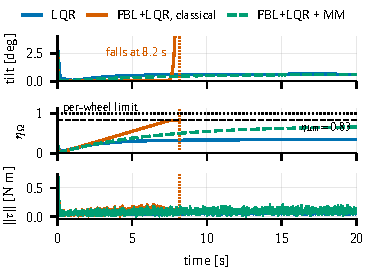
\includegraphics[width=0.72\columnwidth]{figures/fig_timeseries.pdf}
\caption{Corner balancing with a \SI{2}{\milli\metre} center-of-mass offset.
The classical FBL+LQR design (orange) tracks attitude until the
torque--speed envelope exhausts its accelerating authority, then falls; the same
design with momentum management (green, dashed) holds a small tilt that bleeds
the wheels through gravity. Middle: component-wise budget index
$\eta_\Omega=\max_i|\Omega_i|/\Omega_{\max}$: per-wheel limit dotted,
friction--envelope limit $\eta_{\lim}$ dashed. Tilt axis clipped at
\SI{4}{\degree}.}
\label{fig:timeseries}
\end{figure}

\subsection{Integral action on attitude does not rescue them}

A persistent disturbance is textbook integral territory, so a comparison in
which the nonlinear laws have no integrator would be rigged. Every design
therefore has an integral variant, tuned by the same protocol. It does not
help: over \mcSeeds{} perturbed plants the balanced-run
rate moves from \fblMcCl{} to \fblMcInt\,\si{\percent} for FBL+LQR,
\smcMcCl{} to \smcMcInt\,\si{\percent} for SMC and \backsteppingMcCl{} to
\backsteppingMcInt\,\si{\percent} for backstepping, and for the LQR it \emph{falls},
from \lqrMcCl{} to \lqrMcInt\,\si{\percent}. The PID already integrates.

The reason is exact: an unsaturated integrator on $\btheta_e$ makes
$\btheta_e=0$ the only candidate rest point, which
Proposition~\ref{prop:lean}(i) excludes when $P\btau_d\neq0$, so momentum ramps
at $P\btau_d$ whatever the gains. Integral action on stored momentum is a
different design, not tested here.

In these runs the classical designs never reach the wheel-speed limit. They fail at
$\eta_\Omega\approx\etaFall$, the terminal speed at which the accelerating
envelope \eqref{eq:envelope} only just covers bearing friction
($\eta_\Omega=\etaLim$, Sec.~\ref{sec:mm}); a model with only a hard speed
clamp would have predicted a longer survival. Fig.~\ref{fig:sweeps}
sweeps the asymmetry and the momentum budget. Sweeping $\Omega_{\max}$, the LQR balances down to
\lqrMinOmegaCl\,\si{\radian\per\second} while no classical nonlinear design
balances at \emph{any} budget in the swept range: their failure is not having
too little momentum but never releasing what they store. With the augmentation
they need \mmMinOmegaLo--\mmMinOmegaHi\,\si{\radian\per\second}.

\begin{figure}[t]
\centering
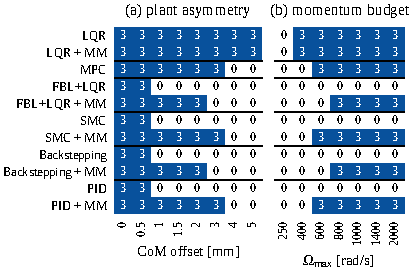
\includegraphics[width=0.80\columnwidth]{figures/fig_sweeps.pdf}
\caption{Runs that balance, out of 3 (sensor-noise seeds, \SI{3}{\degree}
initial tilt, \SI{20}{\second}), against (a)~the offset at
$\Omega_{\max}=\SI{1000}{\radian\per\second}$ and (b)~$\Omega_{\max}$ at
\SI{2}{\milli\metre} offset, without and with momentum management (MM).}
\label{fig:sweeps}
\end{figure}

\subsection{The signature of the invariant}

Fig.~\ref{fig:roa} maps recovery over initial tilt and pre-stored wheel momentum
(\SI{1}{\milli\metre} offset, \SI{25}{\second}),
separating momentum stored perpendicular to the balancing axis, which gravity
can dump, from momentum along the axis, which by Lemma~\ref{thm:invariant} it
cannot. Classical FBL+LQR, SMC, backstepping and PID recover \roaBlindCl\,\si{\percent} of the
sampled grid: at this offset they fall within the horizon from any initial state.

The invariant shows itself in how the augmented recovery depends on what is
already stored. With no stored momentum the two directions are
indistinguishable (\roaPerpZero{} against \roaVertZero\,\si{\percent}), as they must
be. Pooled over the five managed designs, as the pre-stored momentum grows the dumpable direction is unaffected
(\roaPerpHigh\,\si{\percent} beyond \SI{60}{\percent} of the budget) while recovery
along the invariant falls to \roaVertHigh\,\si{\percent}.

\begin{figure}[t]
\centering
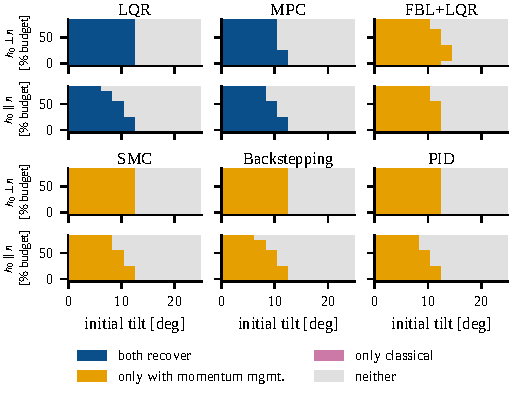
\includegraphics[width=0.75\columnwidth]{figures/fig_roa.pdf}
\caption{Empirical recovery map over initial tilt and pre-stored wheel
momentum $h_0$ (\SI{1}{\milli\metre} offset, \SI{25}{\second}, one seed per cell; not a
certified region of attraction):
momentum stored perpendicular to $\boldsymbol n$ (dumpable) above momentum
along $\boldsymbol n$ (the invariant of Lemma~\ref{thm:invariant}). Orange marks
states only the momentum-managed variant recovers: a band that does not shrink
with dumpable momentum and narrows as momentum along the invariant grows. MPC
has one variant (blue or grey). No cell is pink: on the sampled grid the augmentation never costs
a state the classical design already recovered.}
\label{fig:roa}
\end{figure}

\subsection{Perturbed plants, and a constrained benchmark}

Table~\ref{tab:main} reports \mcSeeds{} plants with
$\pm\SI{20}{\percent}$ on geometry, mass and dissipation parameters and a
center-of-mass offset
drawn per plant from $\mathcal{N}(1,1.5^2)$\,\si{\milli\metre} clipped at
$3\sigma$ (either sign). Episodes
last \mcHorizon\,\si{\second}, so survival is horizon-censored: every
momentum-blind survivor has $|d|\le\clSurvMaxOffset$\,\si{\milli\metre}, and managed
designs near their standing-momentum limit can also fall later. With the inertias recomputed from the drawn geometry, $h_{\max}$ varies by $-\SI{55}{\percent}/+\SI{40}{\percent}$ even though $\Omega_{\max}$ is fixed.

The three momentum-blind designs balance \backsteppingMcCl--\fblMcCl\,\si{\percent} of
plants. The LQR and the MPC weight stored momentum and the PID integrates, so none of
them is momentum-blind. With
momentum management, SMC reaches \smcMcMm\,\si{\percent}, PID
\pidMcMm\,\si{\percent}, backstepping \backsteppingMcMm\,\si{\percent} and
FBL+LQR \fblMcMm\,\si{\percent}. The MPC, with no
augmentation, reaches \mpcMcCl\,\si{\percent}. The LQR reaches
\lqrMcCl\,\si{\percent} on its own; adding the augmentation takes it to
\lqrMcMm\,\si{\percent}, a difference that is \emph{not} significant
(McNemar $p=1$); its tuned $k_h=\lqrKh$ makes the two variants nearly the same
controller. With the survival-first re-tuning of Sec.~\ref{sec:tuning} the
classical rates stay at \lexClLo--\lexClHi\,\si{\percent}, MPC at
\lexMpc\,\si{\percent}, the LQR moves to \lexLqrCl\,\si{\percent} (\lexLqrP),
and momentum management reaches \lexFblMm, \lexBksMm, \lexSmcMm{} and
\lexPidMm\,\si{\percent} for FBL+LQR, backstepping, SMC and PID (the first two
up from \fblMcMm{} and \backsteppingMcMm\,\si{\percent}, \lexFblP, McNemar; one optimizer run per design):
the gain comes from a larger $k_h$ (\num{0.16}$\to$\num{0.26} for FBL+LQR),
paid for in attitude error; exchanging $k_h$ alone reproduces it, so managed
survival is set mainly by $k_h$.
Table~\ref{tab:main} keeps the gains of the submitted study.

On paired plants (McNemar; hierarchical win ratio: survival, accuracy, time to
fall) momentum management wins \num{1.8}--\num{2.0} pairs per loss on FBL+LQR,
SMC, backstepping and PID ($p<10^{-3}$, Holm over fifteen tests). Where
both survive it is \emph{less} accurate (rank-biserial $r>0.85$): it pays for
survival with a permanent tilt.


\begin{table}[t]
\caption{Nominal and Monte-Carlo metrics, with Wilson \SI{95}{\percent}
intervals; Monte-Carlo rates depend on the offset distribution.
$^\dagger$median over runs that balanced.}
\label{tab:main}
\centering
\scriptsize
\input{table_main}
\end{table}

\subsection{What the MPC baseline settles}

With the submitted gains the MPC outperforms managed FBL+LQR and backstepping
(22/0 and 17/0 discordant plants, McNemar $p<10^{-4}$) and ties managed SMC and
PID; after the re-tuning all are level. Momentum management buys no survival
advantage over the MPC. We make no computational claim.

The MPC never reaches its momentum bound (peak \num{858} of
\SI{1000}{\radian\per\second}): like the LQR, it is consistent with surviving through the lean its weight on
stored momentum induces; each of its five falls follows 16--18 solver
fallbacks. What
\eqref{eq:mm} adds is retrofit --- a reference offset leaving the inner loop
untouched --- which takes a PID from \pidMcCl{} to \pidMcMm\,\si{\percent}, level
with the MPC.

\subsection{Limitations}

Sweeping $b_p$ over three decades leaves the unloaded momentum identical to three
significant figures: the unloading is gravity, not pivot dissipation.
Four limitations bound the conclusions. The pivot is an ideal spherical joint
\ref{a:pivot}; a real vertex adds stiction, which widens the equilibrium of
Proposition~\ref{prop:lean} into $\theta^\star\pm\tau_s/(Mgl)$, adds a drilling
torque that breaks Lemma~\ref{thm:invariant}, and can slip.
The effect that does bite at this scale is a \emph{constant}
attitude-estimate bias $b$: since any equilibrium holds the true gravity-balance
attitude (Proposition~\ref{prop:lean}), \eqref{eq:mm} absorbs it as additional
standing momentum, to first order $Mgl\|Pb\|/k_h$, while a design regulating the
measured error to zero meets it as an offset. A bias of \SI{0.64}{\degree} is
torque-equivalent to the whole \SI{2}{\milli\metre} offset studied here, and
IMU-to-diagonal alignment on this class of machine is of that order. We model neither an estimator nor such a bias. No design can unload a
disturbance along $\bn$. The recoveries need pivot friction up to
$\mu\approx0.35$; $\eta_{\lim}$ depends on the unidentified bearing friction
(0.62 at $3b_w$); a \SI{1.1}{\percent} parallel-axis inertia omission changes
none of 120 paired outcomes. The nominal study is in-sample (a tuning scenario). And the study is entirely simulation-based.


\section{Conclusions}
\label{sec:conclusions}

On a corner-balancing Cubli the wheels run out of speed before torque, and only
the destabilizing gravity torque can unload them. Every equilibrium of the
disturbed plant holds a gravity-balanced lean, momentum along $\boldsymbol n$
cannot be unloaded with an ideal pivot, and the sustainable speed is set by
$\eta_{\lim}$, not by $\Omega_{\max}$. In simulation, designs that regulate
the attitude error to zero fail under a millimetre-scale offset, while a
gravity-torque unloading law, the momentum-weighted LQR and the MPC survive by
holding a lean; the augmentation does not outperform the latter two. These
rates are specific to the simulated plants, offsets and horizon; certified
recovery regions, vertex friction and experiments remain open.

\section*{Reproducibility}
Plant, controllers, tuning and Monte-Carlo scripts, per-run results with their
seeds, the supplementary tables and the scripts that regenerate every number,
table and figure (e.g.\ \texttt{make\_numbers.py}) are available at
\url{https://github.com/JoseSegundoM/cubli_momentum_budget}.

\scriptsize
\bibliographystyle{IEEEtran_doi}
\bibliography{refs}

\end{document}
.
% Requires \PaperTitle, \PaperAuthors (UTF-8, hyperref) and \PaperAuthorsPDF
% (PDFDocEncoding octal escapes, \pdfinfo) to be defined first.
\ifdefined\PDFPROFILE\else\def\PDFPROFILE{ieee}\fi
\def\profileinteractive{interactive}
\usepackage{tikz}
\usetikzlibrary{svg.path}
\definecolor{orcidlogocol}{HTML}{A6CE39}
% ORCID iD logo, same artwork as the orcidlink package (vector, no Type 3).
\newlength{\orcidxheight}
\newcommand{\orcidlogo}{\setlength{\orcidxheight}{\fontcharht\font`X}%
  \mbox{\begin{tikzpicture}[yscale=-0.00390625*\orcidxheight,
      xscale=0.00390625*\orcidxheight,transform shape]
    \fill[orcidlogocol] svg{M256,128c0,70.7-57.3,128-128,128C57.3,256,0,198.7,0,128C0,57.3,57.3,0,128,0C198.7,0,256,57.3,256,128z};
    \fill[white] svg{M86.3,186.2H70.9V79.1h15.4v48.4V186.2z}
      svg{M108.9,79.1h41.6c39.6,0,57,28.3,57,53.6c0,27.5-21.5,53.6-56.8,53.6h-41.8V79.1z M124.3,172.4h24.5c34.9,0,42.9-26.5,42.9-39.7c0-21.5-13.7-39.7-43.7-39.7h-23.7V172.4z}
      svg{M88.7,56.8c0,5.5-4.5,10.1-10.1,10.1c-5.6,0-10.1-4.6-10.1-10.1c0-5.6,4.5-10.1,10.1-10.1C84.2,46.7,88.7,51.3,88.7,56.8z};
  \end{tikzpicture}}}
\ifx\PDFPROFILE\profileinteractive
  \usepackage[colorlinks=true,linkcolor=black,citecolor=black,urlcolor=blue,
              bookmarks=false]{hyperref}
  \hypersetup{pdftitle={\PaperTitle},pdfauthor={\PaperAuthors}}
  \newcommand{\orcid}[1]{\href{https://orcid.org/#1}{\orcidlogo}}
  \newcommand{\authoremail}[1]{\href{mailto:#1}{#1}}
  \newcommand{\doititle}[2]{\href{https://doi.org/#1}{#2}}
  \newcommand{\urltitle}[2]{\href{#1}{#2}}
\else
  \pdfinfo{/Title (\PaperTitle) /Author (\PaperAuthorsPDF)}
  \newcommand{\orcid}[1]{\orcidlogo}
  \newcommand{\authoremail}[1]{#1}
  \newcommand{\doititle}[2]{#2}
  \newcommand{\urltitle}[2]{#2}
\fi

\usetikzlibrary{patterns,positioning}
% Coauthor ORCID iDs (found in the BLADE_mars_coaxial CITATION.cff and on
% orcid.org) are shown only after each coauthor confirms them personally.
\newif\ifcoauthororcid \coauthororcidtrue
\newcommand{\coorcid}[1]{\ifcoauthororcid\,\orcid{#1}\fi}
% Affiliation confirmed by the corresponding author (2026-10-23) for all authors.
\newcommand{\paperaffiliation}{Universidad Nacional de Ingenier\'ia (UNI), Faculty of
  Mechanical Engineering, Lima, Peru}


\def\BibTeX{{\rm B\kern-.05em{\sc i\kern-.025em b}\kern-.08em T\kern-.1667em\lower.7ex\hbox{E}\kern-.125emX}}

\newtheorem{lemma}{Lemma}
\newtheorem{theorem}{Theorem}
\newtheorem{proposition}{Proposition}
\theoremstyle{definition}
\newtheorem{definition}{Definition}
\theoremstyle{plain}
\newtheorem{corollary}{Corollary}
\newtheorem{remark}{Remark}

\newcommand{\R}{\mathbb{R}}
\newcommand{\SO}{\mathrm{SO}(3)}
\newcommand{\skewm}[1]{\left[#1\right]_\times}
\newcommand{\bw}{\boldsymbol{\omega}}
\newcommand{\bOm}{\boldsymbol{\Omega}}
\newcommand{\btau}{\boldsymbol{\tau}}
\newcommand{\bh}{\boldsymbol{h}}
\newcommand{\bJ}{\boldsymbol{J}}
\newcommand{\bn}{\boldsymbol{n}}
\newcommand{\bre}{\boldsymbol{r}}
\newcommand{\btheta}{\boldsymbol{\theta}}

% Generated by scripts/make_numbers.py -- do not edit by hand.
% Every numeric value in main.tex comes from here.
\newcommand{\Ja}{1.50}
\newcommand{\backsteppingCICl}{[27, 43]}
\newcommand{\backsteppingCIInt}{[28, 44]}
\newcommand{\backsteppingCIMm}{[78, 91]}
\newcommand{\backsteppingCpu}{355}
\newcommand{\backsteppingCritOffsetCl}{1.0}
\newcommand{\backsteppingCritOffsetMm}{3.0}
\newcommand{\backsteppingFallTime}{8.1}
\newcommand{\backsteppingMcCl}{34.7}
\newcommand{\backsteppingMcInt}{35.3}
\newcommand{\backsteppingMcMm}{85.3}
\newcommand{\backsteppingMinOmegaCl}{n/a}
\newcommand{\backsteppingMinOmegaMm}{800}
\newcommand{\backsteppingNomBudget}{13}
\newcommand{\backsteppingNomSettle}{0.06}
\newcommand{\backsteppingRoaCl}{0}
\newcommand{\backsteppingRoaMm}{45}
\newcommand{\bpSurvivalSpread}{0}
\newcommand{\capacityAxis}{0.260}
\newcommand{\clSurvMaxOffset}{1.13}
\newcommand{\dtErr}{0.67}
\newcommand{\edge}{15}
\newcommand{\energyErr}{$8.9\times 10^{-13}$}
\newcommand{\etaFall}{0.83}
\newcommand{\etaLim}{0.831}
\newcommand{\etaPredErr}{3}
\newcommand{\etaPredErrNoise}{10}
\newcommand{\etaSlopeBks}{0.31}
\newcommand{\etaSlopeFbl}{0.34}
\newcommand{\etaSlopeLqr}{0.17}
\newcommand{\etaSlopePid}{0.20}
\newcommand{\etaSlopeSmc}{0.24}
\newcommand{\fblCICl}{[28, 44]}
\newcommand{\fblCIInt}{[28, 44]}
\newcommand{\fblCIMm}{[75, 88]}
\newcommand{\fblCpu}{354}
\newcommand{\fblCritOffsetCl}{1.0}
\newcommand{\fblCritOffsetMm}{3.0}
\newcommand{\fblFallTime}{8.2}
\newcommand{\fblFirstFallMm}{2.5}
\newcommand{\fblMcCl}{36.0}
\newcommand{\fblMcInt}{36.0}
\newcommand{\fblMcMm}{82.0}
\newcommand{\fblMinOmegaCl}{n/a}
\newcommand{\fblMinOmegaMm}{800}
\newcommand{\fblNomBudget}{17}
\newcommand{\fblNomSettle}{0.06}
\newcommand{\fblRoaCl}{0}
\newcommand{\fblRoaMm}{49}
\newcommand{\fs}{500}
\newcommand{\gravTorqueTen}{0.35}
\newcommand{\hmax}{0.150}
\newcommand{\hzDrift}{$1.1\times 10^{-11}$}
\newcommand{\jacErr}{$7.5\times 10^{-9}$}
\newcommand{\leanErr}{2}
\newcommand{\leanTwoMm}{0.64}
\newcommand{\lever}{14.6}
\newcommand{\lexBksMm}{98.0}
\newcommand{\lexBksP}{$p<10^{-4}$}
\newcommand{\lexClHi}{35.3}
\newcommand{\lexClLo}{31.3}
\newcommand{\lexFblMm}{96.0}
\newcommand{\lexFblP}{$p<10^{-4}$}
\newcommand{\lexLqrCl}{96.7}
\newcommand{\lexLqrP}{McNemar $p=0.12$}
\newcommand{\lexMpc}{96.7}
\newcommand{\lexPidMm}{98.7}
\newcommand{\lexSmcMm}{96.0}
\newcommand{\lqrCICl}{[96, 100]}
\newcommand{\lqrCIInt}{[81, 92]}
\newcommand{\lqrCIMm}{[97, 100]}
\newcommand{\lqrCpu}{189}
\newcommand{\lqrCritOffsetCl}{n/a}
\newcommand{\lqrCritOffsetMm}{n/a}
\newcommand{\lqrFallTime}{n/a}
\newcommand{\lqrKh}{0.002}
\newcommand{\lqrMcCl}{99.3}
\newcommand{\lqrMcInt}{87.3}
\newcommand{\lqrMcMm}{100.0}
\newcommand{\lqrMinOmegaCl}{400}
\newcommand{\lqrMinOmegaMm}{400}
\newcommand{\lqrNomBudget}{9}
\newcommand{\lqrNomSettle}{0.08}
\newcommand{\lqrRoaCl}{45}
\newcommand{\lqrRoaMm}{45}
\newcommand{\mass}{1.41}
\newcommand{\mcHorizon}{15}
\newcommand{\mcSeeds}{150}
\newcommand{\mmMinOmegaHi}{800}
\newcommand{\mmMinOmegaLo}{600}
\newcommand{\mpcCICl}{[92, 99]}
\newcommand{\mpcCpu}{221}
\newcommand{\mpcMcCl}{96.7}
\newcommand{\mpcNomBudget}{9}
\newcommand{\mpcNomSettle}{0.08}
\newcommand{\omegaTerm}{831}
\newcommand{\omegamax}{1000}
\newcommand{\pidCICl}{[26, 42]}
\newcommand{\pidCIInt}{[26, 42]}
\newcommand{\pidCIMm}{[92, 99]}
\newcommand{\pidCpu}{196}
\newcommand{\pidCritOffsetCl}{1.0}
\newcommand{\pidCritOffsetMm}{4.0}
\newcommand{\pidFallTime}{7.9}
\newcommand{\pidMcCl}{33.3}
\newcommand{\pidMcInt}{33.3}
\newcommand{\pidMcMm}{96.7}
\newcommand{\pidMinOmegaCl}{n/a}
\newcommand{\pidMinOmegaMm}{600}
\newcommand{\pidNomBudget}{14}
\newcommand{\pidNomSettle}{0.06}
\newcommand{\pidRoaCl}{0}
\newcommand{\pidRoaMm}{46}
\newcommand{\roaBlindCl}{0}
\newcommand{\roaPerpCl}{16}
\newcommand{\roaPerpHigh}{49}
\newcommand{\roaPerpMm}{50}
\newcommand{\roaPerpZero}{50}
\newcommand{\roaVertCl}{14}
\newcommand{\roaVertHigh}{34}
\newcommand{\roaVertMm}{42}
\newcommand{\roaVertZero}{50}
\newcommand{\satTime}{0.43}
\newcommand{\smcCICl}{[28, 44]}
\newcommand{\smcCIInt}{[28, 44]}
\newcommand{\smcCIMm}{[88, 97]}
\newcommand{\smcCpu}{365}
\newcommand{\smcCritOffsetCl}{1.0}
\newcommand{\smcCritOffsetMm}{4.0}
\newcommand{\smcFallTime}{8.2}
\newcommand{\smcMcCl}{36.0}
\newcommand{\smcMcInt}{36.0}
\newcommand{\smcMcMm}{94.0}
\newcommand{\smcMinOmegaCl}{n/a}
\newcommand{\smcMinOmegaMm}{600}
\newcommand{\smcNomBudget}{12}
\newcommand{\smcNomSettle}{0.06}
\newcommand{\smcRoaCl}{0}
\newcommand{\smcRoaMm}{46}
\newcommand{\swingBalanced}{0/5}
\newcommand{\swingGamma}{0.07}
\newcommand{\taumax}{0.50}
\newcommand{\tsatPred}{15.6}
\newcommand{\tsatSlope}{16.5}


\renewcommand{\topfraction}{0.92}
\renewcommand{\bottomfraction}{0.85}
\renewcommand{\textfraction}{0.07}
\renewcommand{\floatpagefraction}{0.80}
\setlength{\textfloatsep}{7pt plus 2pt minus 2pt}
\setlength{\floatsep}{7pt plus 2pt minus 2pt}
\setlength{\intextsep}{7pt plus 2pt minus 2pt}
\setlength{\abovecaptionskip}{3pt}
\setlength{\belowcaptionskip}{0pt}

\begin{document}

\title{Gravity-Torque Momentum Management for a\\
Three-Wheel Reaction-Wheel Inverted Pendulum}

\author{\IEEEauthorblockN{Jose Luis Segundo Manayay\textsuperscript{*}\,\orcid{0009-0002-9203-8710},
Javier Yanpier Garay Yovera\coorcid{0009-0001-1645-8724},
Francisco Jes\'us Rodr\'iguez Huiman\coorcid{0009-0006-6972-2484}}
\IEEEauthorblockA{\paperaffiliation\\
\authoremail{jose.segundo.m@uni.pe}; \authoremail{javier.garay.y@uni.pe}; \authoremail{francisco.rodriguez.h@uni.pe}\\
{\footnotesize $^{*}$Corresponding author}}}

\maketitle
\raggedbottom

\begin{abstract}
A reaction wheel that holds a body against a persistent torque integrates that
torque, so its speed, not its torque, is what runs out. On a pendulum balancing
about a ground pivot the only external torque that can unload the wheels is
gravity, which also destabilizes the plant. We show that any equilibrium of the
disturbed plant holds the attitude at which gravity balances the disturbance,
with no momentum accumulating in the wheels, so designs that regulate the
attitude error to zero have no equilibrium to reach. A \SI{2}{\milli\metre}
center-of-mass offset needs under \SI{1}{\degree} of lean, yet it fells
feedback linearization, sliding mode control, backstepping and PID, and an
integrator on the attitude error does not help. On a nonlinear three-wheel
model with a torque--speed envelope, a digital loop and sensor noise, over
\mcSeeds{} simulated plants with random center-of-mass offsets and a
\mcHorizon\,\si{\second} horizon, these
designs balance \pidMcCl--\fblMcCl\,\si{\percent} of the plants; a
gravity-torque unloading augmentation raises them to
\fblMcMm--\pidMcMm\,\si{\percent}; the best is level with a constrained
MPC (\mpcMcCl\,\si{\percent}), and none outperforms it or an LQR weighted on
stored momentum (\lqrMcCl\,\si{\percent}).
\end{abstract}

\begin{IEEEkeywords}
underactuated systems, reaction wheels, inverted pendulum, momentum management,
actuator constraints, model predictive control, sliding mode control,
backstepping
\end{IEEEkeywords}

\section{Introduction}
\label{sec:intro}

The reaction-wheel pendulum is a standard benchmark for nonlinear
control~\cite{spong2001}, and the Cubli~\cite{gajamohan2013,muehlebach2017}
extends it to balancing a cube on one vertex with three orthogonal wheels;
comparisons of LQR, feedback linearization, sliding mode control and
backstepping on this plant are common~\cite{wasiwitono2025}. They usually model
the actuator as a torque saturation. A wheel that holds a body against a
persistent torque, however, \emph{integrates} it, and its speed grows until no
reaction torque is left in that direction; wheel-speed excess is the reported
failure mode on a Cubli-type rover~\cite{huang2022}.

Spacecraft handle this with momentum management~\cite{sidi1997}, unloading the
wheels through an external torque~\cite{powell1972} or constraining wheel
momentum directly~\cite{alipour2025}. For balancing machines, the invariance of
the Cubli's vertical momentum is known~\cite{muehlebach2017}, a ballbot holds a
center-of-mass offset by leaning~\cite{vaidya2015ballbot}, a reaction-wheel
bicycle balances under lateral load~\cite{huang2025bicycle}, and reference
governors enforce constraints through set-points~\cite{garone2017governors}.
What is specific to a body balancing about a ground pivot is that the only
unloading torque is the \emph{same first-order gravity torque} that
destabilizes it: in orbit unloading costs pointing accuracy, here it costs
stability margin.

We ask which designs keep such a pendulum balanced under a persistent
disturbance when wheel speed, not torque, is the binding limit, and contribute:
(i)~an equilibrium condition (Proposition~\ref{prop:lean}): every equilibrium of
the disturbed plant holds a gravity-balanced lean, to first order
$\|P\btau_d\|/(Mgl)$, so designs regulating $\btheta_e\!\to\!0$ have no
equilibrium to reach; (ii)~a directional capacity bound
(Proposition~\ref{prop:capacity}; cf.~\cite{markley2009envelopes}) that corrects
the scalar budget by $\|\bn\|_1$; (iii)~a measurement of which limit binds:
classical designs fail at $\eta_\Omega\approx\etaFall$, where the accelerating
envelope no longer covers bearing friction; and (iv)~a comparison of five
designs, each classical, with integral action and with momentum management,
against a constrained MPC, all tuned by one protocol
(Secs.~\ref{sec:control}--\ref{sec:results}).

\section{Problem Formulation}
\label{sec:model}

\subsection{Geometry and states}

The testbed is a cube of edge $L$ carrying three identical reaction wheels
whose spin axes coincide with the body axes $\bre_1,\bre_2,\bre_3$
(Fig.~\ref{fig:system}). It pivots about one vertex, treated as an ideal
spherical joint. Let $R\in\SO$ rotate body coordinates into the inertial
frame, $\bw\in\R^3$ be the body angular velocity, and $\bOm\in\R^3$ collect
the wheel speeds \emph{relative to the body}.

Let $\bJ$ be the inertia of the whole assembly about the pivot, wheels
included as if rigidly attached, $\bJ_w=J_a I_3$ the wheel axial inertias, and
$\bJ_b=\bJ-\bJ_w$. The total angular momentum about the pivot, in body
coordinates, is
\begin{equation}
\bh = \bJ\bw + \bJ_w\bOm .
\label{eq:momentum}
\end{equation}

\subsection{Equations of motion}

Wheel torques are internal, so the only external actions about the pivot are
gravity and pivot friction. Writing $\btau_g(R)=M\,\bre_c\times R^{\!\top}\!
\boldsymbol{g}$ for the gravity torque, with $\bre_c$ the vector from pivot to
center of mass,
\begin{align}
\bJ\dot\bw + \bJ_w\dot\bOm &= \btau_g(R) - \bw\times\bh - b_p\,\bw ,
\label{eq:euler}\\
\bJ_w(\dot\bOm + \dot\bw) &= \btau - \btau_f(\bOm) ,
\label{eq:wheel}
\end{align}
where $\btau$ are the wheel torques and $\btau_f$ collects viscous and Coulomb
bearing friction. Eliminating $\dot\bOm$ gives the form that is integrated,
\begin{align}
\bJ_b\dot\bw &= \btau_g(R) - \bw\times\bh - b_p\bw - \btau + \btau_f ,
\label{eq:wdot}\\
\dot\bOm &= \bJ_w^{-1}\!\left(\btau - \btau_f\right) - \dot\bw ,
\label{eq:Omdot}\\
\dot R &= R\,\skewm{\bw} .
\label{eq:kin}
\end{align}
No small-angle approximation is made; the attitude is propagated as a unit
quaternion. Setting $\btau=0$ and all friction to zero renders the system
conservative, which is the first of the verification tests reported in
Sec.~\ref{sec:verif}.

\subsection{Actuator and implementation model}
\label{sec:actuator}

Three limits act on the commanded torque, and they are not interchangeable.
Besides the peak torque $|\tau_i|\le\tau_{\max}$ and a slew-rate limit, a
brushless drive obeys a torque--speed envelope: the torque available in the
\emph{accelerating} direction decays as the wheel approaches $\Omega_{\max}$,
\begin{equation}
\tau_i^{\text{avail}}(\Omega_i) = \tau_{\max}
\max\!\left(0,\,1-\frac{|\Omega_i|}{\Omega_{\max}}\right) ,
\label{eq:envelope}
\end{equation}
while braking torque remains fully available. The controller runs at
$f_s=\fs{}$\,\si{\hertz} with zero-order hold and no computation delay;
the wheel speed is reconstructed from a quantized encoder and the rates
come from a gyro with white noise and a per-run bias. All results below are
obtained in this digital loop, not in continuous time with exact state
feedback.

\subsection{Standing assumptions and control objective}
\label{sec:assumptions}

\begin{enumerate}[label=(A\arabic*),leftmargin=*]
\item \label{a:pivot} The vertex contact is an ideal spherical joint: it
      transmits no torque about the pivot other than viscous friction
      $-b_p\bw$ with $b_p\ge0$, and the contact does not slip.
\item \label{a:rigid} Body and wheels are rigid; each wheel is balanced and
      axisymmetric about its spin axis, and the three spin axes coincide with
      the body axes.
\item \label{a:act} The delivered torque respects \eqref{eq:envelope}, the
      peak torque and the slew limit.
\item \label{a:meas} Attitude and body rates are available at $f_s$ with
      white Gaussian noise and a constant per-run gyro bias, and the controller knows the plant
      parameters only up to a bounded multiplicative uncertainty and an unknown
      center-of-mass offset. No estimator is modelled and no constant
      attitude-estimate bias is included.
\end{enumerate}

\begin{definition}[Constrained balancing]
\label{def:objective}
Given \ref{a:pivot}--\ref{a:meas}, design $\btau(\cdot)$ such that, from
initial conditions in a set $\mathcal{S}$, attitude and body rate converge to
an admissible equilibrium ($|\Omega_i|\le\Omega_{\max}$; only
$\eta_\Omega\le\etaLim$ is attainable, Sec.~\ref{sec:mm}) on the level set of
the vertical momentum $\boldsymbol{e}_z^{\!\top}R\bh$ fixed by the initial
condition (slowly drifting if $b_p>0$), \emph{and}
$|\Omega_i(t)|\le\Omega_{\max}$ for all $t\ge0$ and all $i$.
\end{definition}

Convergence is asked of a level set, not of an isolated point, because that
momentum is conserved (Lemma~\ref{thm:invariant}) and cannot be regulated
(Corollary~\ref{cor:uncontrollable}). The simulations below evaluate
finite-horizon recovery; they do not certify this property.
Definition~\ref{def:objective} scopes this paper to local balancing and
momentum management about the corner equilibrium; global swing-up and its
handover are outside that scope and are assumed to be discharged by a separate
transient controller that delivers the state into $\mathcal{S}$. The wheel-speed
constraint is not an implementation detail appended to a stability requirement:
Sec.~\ref{sec:budget} shows it is the binding one.


\begin{figure}[t]
\centering
\begin{tikzpicture}[>=stealth, line cap=round, font=\scriptsize]
\fill[pattern=north east lines, pattern color=black!45] (-1.25,-0.12) rectangle (1.25,0);
\draw[thick] (-1.25,0) -- (1.25,0);
\fill[black!31] (-0.631,0.599) -- (0.000,0.000) -- (0.013,0.643) -- (-0.619,1.242) -- cycle;
\fill[black!32] (0.000,0.000) -- (0.775,0.477) -- (0.788,1.120) -- (0.013,0.643) -- cycle;
\fill[black!17] (0.013,0.643) -- (0.788,1.120) -- (0.157,1.719) -- (-0.619,1.242) -- cycle;
\draw[black, line width=0.6pt] (0.000,0.000) -- (0.013,0.643);
\draw[black, line width=0.6pt] (0.000,0.000) -- (-0.631,0.599);
\draw[black, line width=0.6pt] (0.000,0.000) -- (0.775,0.477);
\draw[black, line width=0.6pt] (0.013,0.643) -- (-0.619,1.242);
\draw[black, line width=0.6pt] (0.013,0.643) -- (0.788,1.120);
\draw[black, line width=0.6pt] (-0.631,0.599) -- (-0.619,1.242);
\draw[black!35, dashed] (-0.631,0.599) -- (0.144,1.076);
\draw[black, line width=0.6pt] (-0.619,1.242) -- (0.157,1.719);
\draw[black, line width=0.6pt] (0.775,0.477) -- (0.788,1.120);
\draw[black!35, dashed] (0.775,0.477) -- (0.144,1.076);
\draw[black, line width=0.6pt] (0.788,1.120) -- (0.157,1.719);
\draw[black!35, dashed] (0.144,1.076) -- (0.157,1.719);
\draw[blue!45!black, fill=blue!7, line width=0.5pt] (-0.549,0.849) -- (-0.545,0.884) -- (-0.536,0.913) -- (-0.521,0.935) -- (-0.501,0.949) -- (-0.475,0.955) -- (-0.446,0.953) -- (-0.414,0.942) -- (-0.379,0.924) -- (-0.342,0.898) -- (-0.304,0.866) -- (-0.267,0.827) -- (-0.231,0.783) -- (-0.196,0.736) -- (-0.164,0.685) -- (-0.136,0.633) -- (-0.112,0.581) -- (-0.093,0.529) -- (-0.080,0.480) -- (-0.072,0.435) -- (-0.069,0.394) -- (-0.073,0.358) -- (-0.083,0.329) -- (-0.098,0.307) -- (-0.118,0.293) -- (-0.143,0.287) -- (-0.172,0.290) -- (-0.205,0.300) -- (-0.240,0.318) -- (-0.277,0.344) -- (-0.314,0.377) -- (-0.352,0.415) -- (-0.388,0.459) -- (-0.423,0.507) -- (-0.454,0.557) -- (-0.482,0.609) -- (-0.506,0.661) -- (-0.525,0.713) -- (-0.539,0.762) -- (-0.547,0.808) -- (-0.549,0.849) -- cycle;
\draw[blue!45!black, fill=blue!7, line width=0.5pt] (0.689,0.741) -- (0.686,0.777) -- (0.676,0.808) -- (0.659,0.833) -- (0.635,0.851) -- (0.606,0.861) -- (0.571,0.864) -- (0.532,0.860) -- (0.490,0.849) -- (0.445,0.830) -- (0.399,0.805) -- (0.353,0.773) -- (0.308,0.737) -- (0.265,0.696) -- (0.225,0.651) -- (0.189,0.605) -- (0.159,0.557) -- (0.134,0.510) -- (0.115,0.463) -- (0.104,0.419) -- (0.099,0.379) -- (0.102,0.343) -- (0.112,0.312) -- (0.129,0.288) -- (0.153,0.270) -- (0.182,0.259) -- (0.217,0.256) -- (0.256,0.260) -- (0.298,0.272) -- (0.343,0.290) -- (0.389,0.316) -- (0.435,0.347) -- (0.481,0.384) -- (0.524,0.425) -- (0.563,0.469) -- (0.599,0.515) -- (0.630,0.563) -- (0.654,0.611) -- (0.673,0.657) -- (0.684,0.701) -- (0.689,0.741) -- cycle;
\draw[->, thick, blue!60!black] (0,0) -- (0.426,0.262);
\node[blue!60!black, fill=white, inner sep=0.5pt] at (0.558,0.343) {$\boldsymbol r_1$};
\draw[->, thick, blue!60!black] (0,0) -- (-0.347,0.329);
\node[blue!60!black, fill=white, inner sep=0.5pt] at (-0.455,0.431) {$\boldsymbol r_2$};
\draw[->, thick, blue!60!black] (0,0) -- (0.007,0.354);
\node[blue!60!black, fill=white, inner sep=0.5pt] at (0.177,0.334) {$\boldsymbol r_3$};
\draw[densely dashed, red!70!black] (0,0) -- (0.185,2.029) node[anchor=south west, inner sep=1pt] {$\boldsymbol n$};
\draw[densely dotted] (0,0) -- (0,2.029) node[anchor=south, inner sep=1pt] {$\boldsymbol e_z$};
\draw[->] (0,1.891) arc[start angle=90, delta angle=-7.00, radius=1.891];
\node[anchor=east, fill=white, inner sep=0.6pt] at (-0.04,1.771) {$\theta^\star$};
\draw[black!60] (0.078,0.860) circle (1.3pt);
\fill (0,0.863) circle (1.3pt);
\draw[black!60, line width=0.3pt] (0,0.863) -- (-0.95,1.113) node[anchor=east, inner sep=1pt, text=black] {CoM};
\draw[->, thick] (0,0.863) -- (0,0.483) node[anchor=west, pos=0.6, fill=white, inner sep=0.6pt] {$M\boldsymbol g$};
\fill (0,0) circle (1.4pt);
\node[anchor=north east, inner sep=2pt] at (-0.05,-0.12) {pivot};
\end{tikzpicture}
\\[-1pt]
{\footnotesize (a)}\\[2pt]
% Fig. 1(b): the closed loop as simulated (Secs. II-C, IV). All designs
% share actuator, plant and sensor models; the momentum manager (14) only shifts
% the attitude reference, e = theta_e - theta_r. (MPC: law and constraints in
% one optimization, no manager.)
\begin{tikzpicture}[>=stealth, x=1mm, y=1mm, font=\scriptsize, line width=0.5pt,
  blk/.style={draw, rounded corners=1pt, align=center, inner sep=1.5pt},
  flow/.style={->, line width=0.6pt}]
\node[draw, circle, inner sep=0pt, minimum size=3.4mm] (s) at (0,0) {};
\node[blk, minimum width=21mm, minimum height=8mm] (law) at (16,0)
  {attitude law\\(5 designs, Sec.~IV)};
\node[blk, minimum width=16mm, minimum height=8mm, fill=black!6] (act) at (42,0)
  {envelope (7)\\$|\tau_i|\le\tau_{\max}$};
\node[blk, minimum width=13mm, minimum height=8mm, fill=black!6] (plant) at (61,0)
  {Cubli\\(2)--(6)};
\node[blk, minimum width=25mm, minimum height=10mm, fill=black!6] (sens) at (47,-12)
  {sensors at $f_s$\\gyro (noise, bias)\\quantized encoder};
\node[blk, minimum width=19mm, minimum height=7mm, fill=orange!14] (mm) at (14,-15)
  {momentum\\manager (14)};
\node[inner sep=1pt] (dist) at (61,9) {$\boldsymbol\tau_d$ (CoM offset)};
\draw[flow] (s) -- node[above] {$e$} (law);
\draw[flow] (law) -- node[above] {$\boldsymbol\tau$} node[below, font=\tiny] {ZOH} (act);
\draw[flow] (act) -- (plant);
\draw[flow, densely dashed] (dist) -- (plant);
\draw[flow] (plant.east) -- (71,0) -- (71,-12) -- (sens.east);
\draw[flow] (34.5,-9) -- (0,-9) -- node[right, pos=0.45, inner sep=1pt] {$\boldsymbol\theta_e$} (s.south);
\draw[flow] (16,-9) -- node[left, pos=0.5, inner sep=1pt] {$\boldsymbol\omega,\boldsymbol\Omega$} (16,-4);
\draw[flow] (34.5,-15) -- node[above] {$\boldsymbol h_w$} (mm.east);
\draw[flow, orange!70!black] (mm.west) -- (-6,-15) -- node[left, pos=0.5] {$\boldsymbol\theta_r$} (-6,0) -- (s.west);
\node[font=\tiny] at (-2.6,2.2) {$-$};
\node[font=\tiny] at (1.9,-3.1) {$+$};
\end{tikzpicture}
\\[-1pt]
{\footnotesize (b)}
\caption{(a)~Idealised side view of the testbed (not to scale): a cube on one
vertex (ideal pivot, \ref{a:pivot}), wheel axes $\bre_1$--$\bre_3$ along the
edges leaving the pivot, and the balancing axis $\boldsymbol n$. At the
equilibrium of Proposition~\ref{prop:lean} under a center-of-mass offset, the
true center of mass (filled) is above the pivot and the geometric center
(open) leans with $\boldsymbol n$ by $\theta^\star$ (exaggerated; at
\SI{2}{\milli\metre}, $\theta^\star=\leanTwoMm\,\si{\degree}$). (b)~Simulated
loop shared by all designs; the momentum manager~(14) only shifts the attitude
reference, and the MPC replaces law and manager.}
\label{fig:system}
\end{figure}

\section{Main Results: the Momentum Budget}
\label{sec:budget}

\begin{lemma}[Momentum invariant and its drift]
\label{thm:invariant}
Consider \eqref{eq:euler}--\eqref{eq:kin} with $b_p\ge0$ and let
$\boldsymbol{e}_z$ be the vertical. Then, for \emph{any} wheel torque
$\btau(\cdot)$,
\begin{equation}
\frac{d}{dt}\!\left(\boldsymbol{e}_z^{\!\top}R\bh\right)
 = -\,b_p\,\boldsymbol{e}_z^{\!\top}R\bw .
\label{eq:drift}
\end{equation}
For an ideal pivot ($b_p=0$) the quantity $\boldsymbol{e}_z^{\!\top}R\bh$ is
therefore constant along every trajectory, and for $b_p>0$ its drift is bounded
by $b_p\int_0^t\|\bw\|\,ds$.
\end{lemma}

\begin{proof}
$\frac{d}{dt}(R\bh)=R(\dot\bh+\bw\times\bh)=R\,\btau_g-b_pR\bw$ by
\eqref{eq:euler}. Since $\btau_g=M\bre_c^{I}\times\boldsymbol{g}$ with
$\boldsymbol{g}\parallel\boldsymbol{e}_z$, we have
$\boldsymbol{e}_z^{\!\top}R\btau_g=0$, which leaves \eqref{eq:drift}. The wheel
torques never appear: they are internal and cancel in \eqref{eq:euler}.
\end{proof}

The invariance is established in~\cite{muehlebach2017}; on the simulated plant
($b_p=\SI{1e-3}{\newton\metre\second\per\radian}$) the drift stays below
\SI{1e-6}{\newton\metre\second} over \SI{20}{\second}, orders of magnitude
less than the momentum Sec.~\ref{sec:mm} moves.

The wheels are a \emph{store}, not a sink. The storable set is the \emph{box}
$\mathcal{H}=\{\bh_w:\|\bh_w\|_\infty\le h_{\max}\}$ with
$h_{\max}=J_a\Omega_{\max}=\hmax{}$\,\si{\newton\metre\second} per wheel, so
saturation is measured component-wise by
$\eta_\Omega:=\max_i|\Omega_i|/\Omega_{\max}=\|\bh_w\|_\infty/h_{\max}$ and
\ref{a:act} reads $\eta_\Omega\le1$. The Euclidean norm is the wrong index:
$\|\bh_w\|_2$ can reach $\sqrt3\,h_{\max}$ inside $\mathcal{H}$.

\begin{proposition}[Directional capacity]
\label{prop:capacity}
For any unit $\bn$,
$\max_{\bh_w\in\mathcal{H}}\bn^{\!\top}\bh_w=h_{\max}\|\bn\|_1$, attained at the
vertex $\Omega_i=\Omega_{\max}\operatorname{sign}(n_i)$. For the corner
equilibrium of a cube, $\bn=(1,1,1)/\sqrt3$ and the capacity along the
balancing axis is $\sqrt3\,h_{\max}=\SI{0.260}{\newton\metre\second}$.
\end{proposition}

\begin{proof}
$\bn^{\!\top}\bh_w=J_a\bn^{\!\top}\bOm$ is linear, so its maximum over a box is
attained at a vertex; evaluating gives $J_a\Omega_{\max}\sum_i|n_i|$.
\end{proof}

\begin{corollary}[Loss of stabilizability]
\label{cor:uncontrollable}
Let $\bn$ be the balancing axis in body coordinates and linearize
\eqref{eq:wdot}--\eqref{eq:kin} about the corner equilibrium with no stored
wheel momentum (or momentum along $\bn$), with states
$z=(\btheta_e,\bw,\bh_w)$, $\bh_w=\bJ_w\bOm$, yaw included. Then for \emph{every} $b_p\ge0$
the row vector
\begin{equation}
v(b_p)=\begin{bmatrix} b_p\,\bn^{\!\top} & (\bJ\bn)^{\!\top} &
\bn^{\!\top}\end{bmatrix}
\label{eq:annih}
\end{equation}
satisfies $v(b_p)A=0$ and $v(b_p)B=0$. Hence $\mathrm{rank}\,[A\;\;B]=n_x-1$,
the uncontrollable eigenvalue is $\lambda_{uc}=0$ exactly, and $(A,B)$ is
\emph{not stabilizable}.
\end{corollary}

\begin{proof}
$vB=0$ because wheel torque enters $\dot\bw$ and $\dot\bh_w$ with equal and
opposite weight, which $(\bJ\bn,\bn)$ annihilates. $vA=0$ states that
$\bn^{\!\top}(\bJ\bw+\bh_w)+b_p\,\bn^{\!\top}\btheta_e$ is conserved to first order: the
friction torque $-b_p\bw$ integrates to $-b_p\btheta_e$, so the momentum it
removes is exactly the $b_p$ term. Thus $v$ is a left eigenvector of $A$ at
$\lambda=0$ and $vB=0$ makes the PBH test fail there; verified numerically to
\num{7e-16} over $b_p\in[0,1]$. With transverse stored momentum $\bh_0$ the
annihilator gains the term $(\bh_0\times\bn)^{\!\top}$ in the attitude block
and the rank deficiency persists.
\end{proof}

As noted in~\cite{gajamohan2013}, pivot friction does \emph{not} restore
stabilizability (with yaw free, $b_p>0$ dissipates vertical momentum only
through net yaw rotation, unused here). An LQR posed on the
full linearization has no stabilizing Riccati solution; every linear design here
is synthesised on the controllable subspace from a Kalman decomposition.


\section{Control design}
\label{sec:control}

Six designs act on the full nonlinear plant and see the same actuator model
and the same measurements: PID, LQR, feedback linearization with an LQR outer
loop (FBL+LQR), sliding mode control (SMC), backstepping and constrained model
predictive control (MPC).

\subsection{Shared cancellation term and notation}

The three nonlinear laws share the cancellation term
\begin{equation}
\Phi(x) = \btau_g(R) - \bw\times\bh - b_p\bw + \btau_f(\bOm),
\label{eq:phi}
\end{equation}
so that \eqref{eq:wdot} reads $\bJ_b\dot\bw=\Phi(x)-\btau$ and the designs
differ in feedback shaping rather than in how much physics each is allowed to
cancel. Let $\btheta_e$ denote the attitude error and $\btheta_r$ a reference
tilt defined in Sec.~\ref{sec:mm}, with $e=\btheta_e-\btheta_r$.

\subsection{Linear-class baselines: PID and LQR}

PID acts on attitude with rate damping and integrator clamping; it is the
declared linear-class baseline. The LQR is a Riccati design on the controllable
subspace of the linearization about the corner equilibrium, with states
$(\btheta_e,\bw,\bh_w)$ and weights $Q=\mathrm{diag}(q_\theta I,q_\omega
I,q_hI)$, $R=rI$. The weight $q_h$ acts directly on stored momentum; this is
what makes the LQR implicitly budget-aware.

\subsection{Feedback linearization with an LQR outer loop}

Cancelling $\Phi(x)$ leaves $\dot\bw=v$ at any attitude for the nominal plant,
and $v$ must still be chosen. The error kinematics are only first order: with
$\btheta_e=2\,\mathrm{vec}(q_e)$ and $q_e=(\eta,\boldsymbol{\epsilon})$ one has
$\dot\btheta_e=\eta\bw+\tfrac12\btheta_e\times\bw$, so $\dot\btheta_e=\bw$ ---
and the double-integrator structure --- holds near the equilibrium (a
\SI{2.6}{\percent} relative error at \SI{3}{\degree}, \SI{39}{\percent} at the
\SI{45}{\degree} fall threshold). The outer loop is the LQR for that double
integrator,
\begin{equation}
v = -(k_1e+k_2\bw), \quad
\btau = \Phi(x)+\bJ_b\!\left(k_1e+k_2\bw\right),
\label{eq:fbl}
\end{equation}
with $(k_1,k_2)$ from the Riccati equation of
$\left(\left[\begin{smallmatrix}0&1\\0&0\end{smallmatrix}\right],
\left[\begin{smallmatrix}0\\1\end{smallmatrix}\right]\right)$ and weights
$(q_\theta,q_\omega,r)$. The wheel speeds are the zero dynamics of the design and
are left unregulated.

\subsection{Sliding mode control}

With sliding variable $s=\bw+\Lambda e$ and boundary layer $\phi$,
\begin{equation}
\btau=\Phi(x)+\bJ_b\!\left(\Lambda\bw+K\,\mathrm{sat}(s/\phi)\right).
\label{eq:smc}
\end{equation}
A boundary layer replaces $\mathrm{sign}$, whose chatter on a sampled loop
would inject momentum.

\subsection{Backstepping}

With $z_1=e$, $\bw_d=-k_1z_1$, $z_2=\bw-\bw_d$ and $\Gamma=\gamma I\succ0$ in
\si{\newton\metre\per\radian} so both terms of
$V=\tfrac12 z_1^{\!\top}\Gamma z_1+\tfrac12 z_2^{\!\top}\bJ_bz_2$ are energies,
\begin{equation}
\btau=\Phi(x)+k_1\bJ_b\bw+K_2z_2+\Gamma z_1
\label{eq:bks}
\end{equation}
gives, for constant $\btheta_r$, $\dot V=-k_1z_1^{\!\top}\Gamma z_1-z_2^{\!\top}K_2z_2+\Delta$ with
$\Delta=\mathcal{O}(\|z\|^3)$ vanishing at $\eta=1$: stability is local.

\subsection{Constrained model predictive control}

MPC solves, nominally every \SI{20}{\milli\second} (about \SI{47}{\hertz}
effective, a floating-point scheduling artefact of our code) over a
\SI{1}{\second} horizon, a quadratic
program in $z$ with $|\tau_i|\le\tau_{\max}$ and $|h_{w,i}|\le h_{\max}$ imposed
on every predicted step and a terminal cost from the discrete Riccati equation
on the controllable subspace. It is the only design here that is \emph{told}
about the momentum limit, although in our runs that bound never becomes active.

Every design except MPC also exists in an \emph{integral} variant (for the PID,
which already integrates, it coincides with the baseline),
$\btau\mathrel{+}=K_i\!\int\!e\,dt$ with clamping, and in a
\emph{momentum-managed} variant defined next.
\subsection{Momentum management}
\label{sec:mm}

Lemma~\ref{thm:invariant} also says how to unload the wheels: since the
wheels cannot remove momentum, an external torque must, and the only one
available is gravity. To first order the gravity torque is
$\btau_g\simeq Mgl(I-\bn\bn^{\!\top})\btheta_e$, so holding the tilt
\begin{equation}
\btheta_r = -\frac{k_h}{Mgl}\,(I-\bn\bn^{\!\top})\,\bh_w
\label{eq:mm}
\end{equation}
produces, to first order, the torque that decelerates the wheels. The commanded lean is clamped at
\SI{3}{\degree}. The projector removes the
component along $\bn$, precisely the one Lemma~\ref{thm:invariant} forbids
removing for $b_p=0$; $k_h=0$ recovers the classical designs, so the augmentation is
measured rather than assumed.

\begin{proposition}[Equilibrium lean and saturation time]
\label{prop:lean}
Let a torque $\btau_d(R)$ act about the pivot. (i)~\emph{(exact)} At any
equilibrium $(R^\star,\bw=0,\bOm^\star)$ of \eqref{eq:wdot}--\eqref{eq:kin},
$\btau_g(R^\star)+\btau_d(R^\star)=0$ and $\btau=\btau_f(\bOm^\star)$: gravity
carries the disturbance, the motors only cover bearing friction, and no
momentum accumulates. (ii)~\emph{(first order, $\bn^{\!\top}\btau_d=0$, small
$\btau_d$)} The tilt part of the equilibrium attitude error satisfies
\begin{equation}
P\btheta^\star = -\frac{1}{Mgl}\,P\,\btau_d ,
\qquad P=I-\bn\bn^{\!\top},
\label{eq:lean}
\end{equation}
(iii)~\emph{(first order, $\bn^{\!\top}\btau_d=0$)} A controller that regulates $\btheta_e\!\to\!0$
admits no equilibrium under $P\btau_d\neq0$: its stored momentum grows as
$\dot\bh_w\simeq P\btau_d$ and, from zero momentum, reaches a saturation index
$\eta^\star$ after
\begin{equation}
t_{sat} \;\simeq\; \frac{\eta^\star h_{\max}}{\|P\btau_d\|_\infty} .
\label{eq:tsat}
\end{equation}
\end{proposition}

\begin{proof}
(i)~With $\bw\equiv0$, \eqref{eq:euler} gives $\bJ_w\dot\bOm=\btau_g+\btau_d$,
which must vanish, and then \eqref{eq:wheel} gives $\btau=\btau_f$.
(ii)~Use $\btau_g\simeq MglP\btheta_e$; the equation is solvable only for
$\btau_d\perp\bn$ (gravity has no torque about $\bn$). (iii)~If
$\btheta_e\equiv0$ then $\btau_g=0$ and, by total momentum,
$\dot\bh_w=\btau_d-\bJ\dot\bw\simeq P\btau_d$.
\end{proof}

For an offset $d$ along a body axis, $\btau_d=-Mgd\,(\boldsymbol{e}_i\times\bn)$, so
$\|P\btau_d\|_2=Mgd\sqrt{2/3}$ and $\|P\btau_d\|_\infty=Mgd/\sqrt3$: the
component of the offset along $\bn$ tilts nothing. The required lean is therefore
$\theta^\star\simeq\sqrt{2/3}\,d/l=\leanTwoMm\,\si{\degree}$ at
$d=\SI{2}{\milli\metre}$ (exactly,
$\operatorname{atan2}(|d|\|P\boldsymbol{e}_i\|,\,l+d\,n_i)$); \eqref{eq:tsat}
takes the \emph{infinity} norm because the budget index is component-wise.
Part~(i) adds a necessary condition: the motor torque on a wheel at the
equilibrium speed, $\tau_f(\Omega^\star)$, is accelerating, so by
\eqref{eq:envelope} $b_w|\Omega_i^\star|+\tau_c\le\tau_{\max}(1-|\Omega_i^\star|/\Omega_{\max})$,
i.e.\ $|\Omega_i^\star|\le\omegaTerm\,\si{\radian\per\second}$
($\eta_\Omega\le\etaLim$) on the nominal plant.

\subsection{Tuning protocol}
\label{sec:tuning}

Every controller is tuned by the same procedure, so that no baseline is
handicapped by its gains: the same cost
\begin{equation}
J_c = \frac{1}{|\mathcal{S}|}\sum_{s\in\mathcal{S}}
\begin{cases}
w_e\!\int\!\|\btheta_e\|\,dt + w_u\!\int\!\|\btau\|^2 dt, & \text{balanced},\\
\rho\,\bigl(1-t_{\text{fall}}/T\bigr), & \text{fallen},
\end{cases}
\label{eq:cost}
\end{equation}
with $w_e=1$, $w_u=20$, $\rho=10^3$: a fallen run is scored by survival time
alone, so truncated error cannot reward failing early. The branches are not
strictly ordered: a fall in the last \SI{2}{\percent} of the horizon can score
below a survival. A survival-first (lexicographic) re-tuning leaves the MPC gains
unchanged and finds no gain set with which a momentum-blind design survives the
asymmetric scenario (Sec.~\ref{sec:results}). The protocol also fixes the same scenario set $\mathcal{S}$ (small and large transients, an asymmetric
plant, a pre-loaded wheel), the same Nelder--Mead optimiser on log-gains and the
same iteration cap, never reached (42--102 cost evaluations per design). All gains are listed in the supplementary material.

\section{Simulation Study}
\label{sec:study}


The testbed is a declared design point, not identified hardware: a
\SI{15}{\centi\metre} cube, $M=\mass\,\si{\kilogram}$, lever
arm $l=\lever\,\si{\centi\metre}$, wheel inertia $J_a=\Ja\times10^{-4}\,
\si{\kilogram\metre\squared}$, $\tau_{\max}=\taumax\,\si{\newton\metre}$ and
$\Omega_{\max}=\omegamax\,\si{\radian\per\second}$, giving
$h_{\max}=\hmax\,\si{\newton\metre\second}$ per wheel; the full parameter
table is in the supplementary material. The model is first checked against properties it
must have: energy conserved to \energyErr{} over \SI{5}{\second} without friction
or torque, the invariant drifting less than \hzDrift{}\,\si{\newton\metre\second}
under arbitrary wheel torques, and the linearization matching a
central-difference Jacobian to \jacErr{}; the step is \SI{1}{\milli\second}
(\dtErr\,\si{\percent} change over $dt\in[0.2,2]\,\si{\milli\second}$).

\label{sec:verif}
The studies sweep the center-of-mass asymmetry, the wheel-speed limit, the peak
torque and the pivot friction; map recovery over initial tilt and pre-stored
momentum in both storage directions; and run \mcSeeds{} plants with
$\pm\SI{20}{\percent}$ on geometry, mass and dissipation parameters (actuator
limits and sensor models fixed) over \mcHorizon\,\si{\second}.
Every controller is designed on the nominal symmetric model; perturbed
parameters enter only the simulated plant. Gains come from
Sec.~\ref{sec:tuning}, tuned at \SI{1.5}{\milli\metre} of offset over
\SI{30}{\second}, an operating point that differs from the Monte Carlo and
appears in Fig.~\ref{fig:sweeps} only as one column.

\section{Results}
\label{sec:results}

% Results section body.  Every number is a macro from numbers.tex, which is
% generated from results/*.csv -- see scripts/make_numbers.py.

From a \SI{3}{\degree} tilt on the nominal plant every controller balances
(\pidNomSettle--\lqrNomSettle\,\si{\second} median time to stay within
\SI{2}{\degree}): this usual regime does not discriminate.

\subsection{A \SI{2}{\milli\metre} asymmetry, and why it is fatal}

Give the plant a \SI{2}{\milli\metre} center-of-mass offset and the classical designs hold attitude perfectly
until they lose the cube (Fig.~\ref{fig:timeseries}). Both halves of
Proposition~\ref{prop:lean} are confirmed numerically. First, the disturbance is
small: the equilibrium lean is
$\theta^\star\simeq\sqrt{2/3}\,d/l=\leanTwoMm\,\si{\degree}$, and with momentum
management the measured steady tilt tracks it to \leanErr\,\si{\percent} over
$d\in[1,3]\,\si{\milli\metre}$ and the wheels stop charging. They stop at a
standing index that a proportional law necessarily leaves and that grows
linearly with $d$: $\etaSlopeFbl$, $\etaSlopeSmc$, $\etaSlopeBks$,
$\etaSlopePid$ and $\etaSlopeLqr$ per mm for FBL+LQR, SMC, backstepping, PID
and LQR (noise-free \SI{60}{\second} runs, nominal plant), within \etaPredErr\,\si{\percent}
(\etaPredErrNoise\,\si{\percent} with sensor noise)
of $Mgd/(\sqrt3\,k_hh_{\max})$ from \eqref{eq:mm} and \eqref{eq:lean} for the
four managed designs (FBL+LQR, SMC, backstepping, PID); FBL+LQR falls from \fblFirstFallMm\,\si{\milli\metre},
where that index exceeds \etaLim. Second,
the classical designs regulate $\btheta_e\!\to\!0$, which is not an equilibrium
of the disturbed plant, so they must supply $P\btau_d$ forever: their stored
momentum ramps linearly and \eqref{eq:tsat} predicts $t_{sat}\propto1/d$. We
measure $t_{sat}d=\tsatSlope\,\si{\second\milli\metre}$ against
\tsatPred\,\si{\second\milli\metre} from \eqref{eq:tsat}.

\begin{figure}[t]
\centering
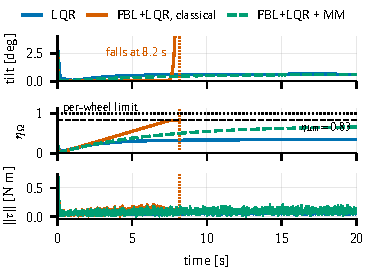
\includegraphics[width=0.72\columnwidth]{figures/fig_timeseries.pdf}
\caption{Corner balancing with a \SI{2}{\milli\metre} center-of-mass offset.
The classical FBL+LQR design (orange) tracks attitude until the
torque--speed envelope exhausts its accelerating authority, then falls; the same
design with momentum management (green, dashed) holds a small tilt that bleeds
the wheels through gravity. Middle: component-wise budget index
$\eta_\Omega=\max_i|\Omega_i|/\Omega_{\max}$: per-wheel limit dotted,
friction--envelope limit $\eta_{\lim}$ dashed. Tilt axis clipped at
\SI{4}{\degree}.}
\label{fig:timeseries}
\end{figure}

\subsection{Integral action on attitude does not rescue them}

A persistent disturbance is textbook integral territory, so a comparison in
which the nonlinear laws have no integrator would be rigged. Every design
therefore has an integral variant, tuned by the same protocol. It does not
help: over \mcSeeds{} perturbed plants the balanced-run
rate moves from \fblMcCl{} to \fblMcInt\,\si{\percent} for FBL+LQR,
\smcMcCl{} to \smcMcInt\,\si{\percent} for SMC and \backsteppingMcCl{} to
\backsteppingMcInt\,\si{\percent} for backstepping, and for the LQR it \emph{falls},
from \lqrMcCl{} to \lqrMcInt\,\si{\percent}. The PID already integrates.

The reason is exact: an unsaturated integrator on $\btheta_e$ makes
$\btheta_e=0$ the only candidate rest point, which
Proposition~\ref{prop:lean}(i) excludes when $P\btau_d\neq0$, so momentum ramps
at $P\btau_d$ whatever the gains. Integral action on stored momentum is a
different design, not tested here.

In these runs the classical designs never reach the wheel-speed limit. They fail at
$\eta_\Omega\approx\etaFall$, the terminal speed at which the accelerating
envelope \eqref{eq:envelope} only just covers bearing friction
($\eta_\Omega=\etaLim$, Sec.~\ref{sec:mm}); a model with only a hard speed
clamp would have predicted a longer survival. Fig.~\ref{fig:sweeps}
sweeps the asymmetry and the momentum budget. Sweeping $\Omega_{\max}$, the LQR balances down to
\lqrMinOmegaCl\,\si{\radian\per\second} while no classical nonlinear design
balances at \emph{any} budget in the swept range: their failure is not having
too little momentum but never releasing what they store. With the augmentation
they need \mmMinOmegaLo--\mmMinOmegaHi\,\si{\radian\per\second}.

\begin{figure}[t]
\centering
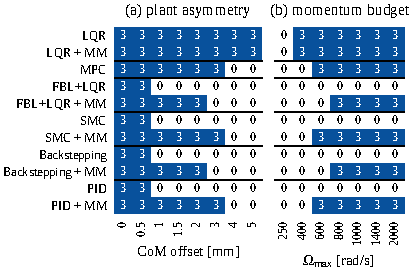
\includegraphics[width=0.80\columnwidth]{figures/fig_sweeps.pdf}
\caption{Runs that balance, out of 3 (sensor-noise seeds, \SI{3}{\degree}
initial tilt, \SI{20}{\second}), against (a)~the offset at
$\Omega_{\max}=\SI{1000}{\radian\per\second}$ and (b)~$\Omega_{\max}$ at
\SI{2}{\milli\metre} offset, without and with momentum management (MM).}
\label{fig:sweeps}
\end{figure}

\subsection{The signature of the invariant}

Fig.~\ref{fig:roa} maps recovery over initial tilt and pre-stored wheel momentum
(\SI{1}{\milli\metre} offset, \SI{25}{\second}),
separating momentum stored perpendicular to the balancing axis, which gravity
can dump, from momentum along the axis, which by Lemma~\ref{thm:invariant} it
cannot. Classical FBL+LQR, SMC, backstepping and PID recover \roaBlindCl\,\si{\percent} of the
sampled grid: at this offset they fall within the horizon from any initial state.

The invariant shows itself in how the augmented recovery depends on what is
already stored. With no stored momentum the two directions are
indistinguishable (\roaPerpZero{} against \roaVertZero\,\si{\percent}), as they must
be. Pooled over the five managed designs, as the pre-stored momentum grows the dumpable direction is unaffected
(\roaPerpHigh\,\si{\percent} beyond \SI{60}{\percent} of the budget) while recovery
along the invariant falls to \roaVertHigh\,\si{\percent}.

\begin{figure}[t]
\centering
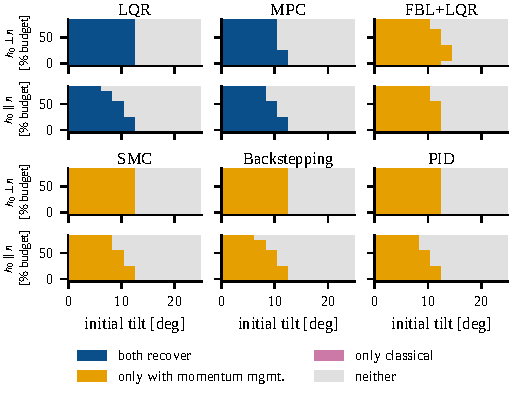
\includegraphics[width=0.75\columnwidth]{figures/fig_roa.pdf}
\caption{Empirical recovery map over initial tilt and pre-stored wheel
momentum $h_0$ (\SI{1}{\milli\metre} offset, \SI{25}{\second}, one seed per cell; not a
certified region of attraction):
momentum stored perpendicular to $\boldsymbol n$ (dumpable) above momentum
along $\boldsymbol n$ (the invariant of Lemma~\ref{thm:invariant}). Orange marks
states only the momentum-managed variant recovers: a band that does not shrink
with dumpable momentum and narrows as momentum along the invariant grows. MPC
has one variant (blue or grey). No cell is pink: on the sampled grid the augmentation never costs
a state the classical design already recovered.}
\label{fig:roa}
\end{figure}

\subsection{Perturbed plants, and a constrained benchmark}

Table~\ref{tab:main} reports \mcSeeds{} plants with
$\pm\SI{20}{\percent}$ on geometry, mass and dissipation parameters and a
center-of-mass offset
drawn per plant from $\mathcal{N}(1,1.5^2)$\,\si{\milli\metre} clipped at
$3\sigma$ (either sign). Episodes
last \mcHorizon\,\si{\second}, so survival is horizon-censored: every
momentum-blind survivor has $|d|\le\clSurvMaxOffset$\,\si{\milli\metre}, and managed
designs near their standing-momentum limit can also fall later. With the inertias recomputed from the drawn geometry, $h_{\max}$ varies by $-\SI{55}{\percent}/+\SI{40}{\percent}$ even though $\Omega_{\max}$ is fixed.

The three momentum-blind designs balance \backsteppingMcCl--\fblMcCl\,\si{\percent} of
plants. The LQR and the MPC weight stored momentum and the PID integrates, so none of
them is momentum-blind. With
momentum management, SMC reaches \smcMcMm\,\si{\percent}, PID
\pidMcMm\,\si{\percent}, backstepping \backsteppingMcMm\,\si{\percent} and
FBL+LQR \fblMcMm\,\si{\percent}. The MPC, with no
augmentation, reaches \mpcMcCl\,\si{\percent}. The LQR reaches
\lqrMcCl\,\si{\percent} on its own; adding the augmentation takes it to
\lqrMcMm\,\si{\percent}, a difference that is \emph{not} significant
(McNemar $p=1$); its tuned $k_h=\lqrKh$ makes the two variants nearly the same
controller. With the survival-first re-tuning of Sec.~\ref{sec:tuning} the
classical rates stay at \lexClLo--\lexClHi\,\si{\percent}, MPC at
\lexMpc\,\si{\percent}, the LQR moves to \lexLqrCl\,\si{\percent} (\lexLqrP),
and momentum management reaches \lexFblMm, \lexBksMm, \lexSmcMm{} and
\lexPidMm\,\si{\percent} for FBL+LQR, backstepping, SMC and PID (the first two
up from \fblMcMm{} and \backsteppingMcMm\,\si{\percent}, \lexFblP, McNemar; one optimizer run per design):
the gain comes from a larger $k_h$ (\num{0.16}$\to$\num{0.26} for FBL+LQR),
paid for in attitude error; exchanging $k_h$ alone reproduces it, so managed
survival is set mainly by $k_h$.
Table~\ref{tab:main} keeps the gains of the submitted study.

On paired plants (McNemar; hierarchical win ratio: survival, accuracy, time to
fall) momentum management wins \num{1.8}--\num{2.0} pairs per loss on FBL+LQR,
SMC, backstepping and PID ($p<10^{-3}$, Holm over fifteen tests). Where
both survive it is \emph{less} accurate (rank-biserial $r>0.85$): it pays for
survival with a permanent tilt.


\begin{table}[t]
\caption{Nominal and Monte-Carlo metrics, with Wilson \SI{95}{\percent}
intervals; Monte-Carlo rates depend on the offset distribution.
$^\dagger$median over runs that balanced.}
\label{tab:main}
\centering
\scriptsize
\setlength{\tabcolsep}{3.0pt}
\begin{tabular}{@{}llrrrcr@{}}
\toprule
& & \multicolumn{2}{c}{Nominal} & \multicolumn{3}{c}{Monte-Carlo} \\
\cmidrule(lr){3-4}\cmidrule(l){5-7}
Controller & Var. & $t_s$ [s] & $\int\|\tau\|^2$ & bal.\ [\%] & 95\,\% CI & IAE$^\dagger$ \\
\midrule
LQR & cl. & 0.08 & 0.010 & 99.3 & [96, 100] & 5.7 \\
LQR & MM & 0.08 & 0.010 & 100.0 & [97, 100] & 5.8 \\
MPC & cl. & 0.08 & 0.015 & 96.7 & [92, 99] & 5.2 \\
FBL+LQR & cl. & 0.06 & 0.102 & 36.0 & [28, 44] & 0.3 \\
FBL+LQR & MM & 0.06 & 0.105 & 82.0 & [75, 88] & 3.4 \\
SMC & cl. & 0.06 & 0.100 & 36.0 & [28, 44] & 0.4 \\
SMC & MM & 0.06 & 0.100 & 94.0 & [88, 97] & 4.7 \\
Backstepping & cl. & 0.06 & 0.131 & 34.7 & [27, 43] & 0.3 \\
Backstepping & MM & 0.06 & 0.131 & 85.3 & [78, 91] & 3.8 \\
PID & cl. & 0.06 & 0.243 & 33.3 & [26, 42] & 0.5 \\
PID & MM & 0.06 & 0.242 & 96.7 & [92, 99] & 5.1 \\
\bottomrule
\end{tabular}
\end{table}

\subsection{What the MPC baseline settles}

With the submitted gains the MPC outperforms managed FBL+LQR and backstepping
(22/0 and 17/0 discordant plants, McNemar $p<10^{-4}$) and ties managed SMC and
PID; after the re-tuning all are level. Momentum management buys no survival
advantage over the MPC. We make no computational claim.

The MPC never reaches its momentum bound (peak \num{858} of
\SI{1000}{\radian\per\second}): like the LQR, it is consistent with surviving through the lean its weight on
stored momentum induces; each of its five falls follows 16--18 solver
fallbacks. What
\eqref{eq:mm} adds is retrofit --- a reference offset leaving the inner loop
untouched --- which takes a PID from \pidMcCl{} to \pidMcMm\,\si{\percent}, level
with the MPC.

\subsection{Limitations}

Sweeping $b_p$ over three decades leaves the unloaded momentum identical to three
significant figures: the unloading is gravity, not pivot dissipation.
Four limitations bound the conclusions. The pivot is an ideal spherical joint
\ref{a:pivot}; a real vertex adds stiction, which widens the equilibrium of
Proposition~\ref{prop:lean} into $\theta^\star\pm\tau_s/(Mgl)$, adds a drilling
torque that breaks Lemma~\ref{thm:invariant}, and can slip.
The effect that does bite at this scale is a \emph{constant}
attitude-estimate bias $b$: since any equilibrium holds the true gravity-balance
attitude (Proposition~\ref{prop:lean}), \eqref{eq:mm} absorbs it as additional
standing momentum, to first order $Mgl\|Pb\|/k_h$, while a design regulating the
measured error to zero meets it as an offset. A bias of \SI{0.64}{\degree} is
torque-equivalent to the whole \SI{2}{\milli\metre} offset studied here, and
IMU-to-diagonal alignment on this class of machine is of that order. We model neither an estimator nor such a bias. No design can unload a
disturbance along $\bn$. The recoveries need pivot friction up to
$\mu\approx0.35$; $\eta_{\lim}$ depends on the unidentified bearing friction
(0.62 at $3b_w$); a \SI{1.1}{\percent} parallel-axis inertia omission changes
none of 120 paired outcomes. The nominal study is in-sample (a tuning scenario). And the study is entirely simulation-based.


\section{Conclusions}
\label{sec:conclusions}

On a corner-balancing Cubli the wheels run out of speed before torque, and only
the destabilizing gravity torque can unload them. Every equilibrium of the
disturbed plant holds a gravity-balanced lean, momentum along $\boldsymbol n$
cannot be unloaded with an ideal pivot, and the sustainable speed is set by
$\eta_{\lim}$, not by $\Omega_{\max}$. In simulation, designs that regulate
the attitude error to zero fail under a millimetre-scale offset, while a
gravity-torque unloading law, the momentum-weighted LQR and the MPC survive by
holding a lean; the augmentation does not outperform the latter two. These
rates are specific to the simulated plants, offsets and horizon; certified
recovery regions, vertex friction and experiments remain open.

\section*{Reproducibility}
Plant, controllers, tuning and Monte-Carlo scripts, per-run results with their
seeds, the supplementary tables and the scripts that regenerate every number,
table and figure (e.g.\ \texttt{make\_numbers.py}) are available at
\url{https://github.com/JoseSegundoM/cubli_momentum_budget}.

\scriptsize
\bibliographystyle{IEEEtran_doi}
\bibliography{refs}

\end{document}
